% !TeX spellcheck = hu_HU
% !TeX encoding = UTF-8
% !TeX program = xelatex
% TODO Change language to en_GB (recommended) or en_US for English documents
\documentclass[11pt,a4paper,oneside]{report}             % Single-side
%\documentclass[11pt,a4paper,twoside,openright]{report}  % Duplex

% thanks to http://tex.stackexchange.com/a/47579/71109
\usepackage{ifxetex}
\usepackage{ifluatex}
\newif\ifxetexorluatex % a new conditional starts as false
\ifnum 0\ifxetex 1\fi\ifluatex 1\fi>0
   \xetexorluatextrue
\fi

\ifxetexorluatex
  \usepackage{fontspec}
\else
  \usepackage[T1]{fontenc}
  \usepackage[utf8]{inputenc}
  \usepackage[lighttt]{lmodern}
\fi

\usepackage[english,magyar]{babel} % Alapértelmezés szerint utoljára definiált nyelv lesz aktív, de később külön beállítjuk az aktív nyelvet.

%\usepackage{cmap}
\usepackage{amsfonts,amsmath,amssymb} % Mathematical symbols.
%\usepackage[ruled,boxed,resetcount,linesnumbered]{algorithm2e} % For pseudocodes. % beware: this is not compatible with LuaLaTeX, see http://tex.stackexchange.com/questions/34814/lualatex-and-algorithm2e
\usepackage{booktabs} % For publication quality tables for LaTeX
\usepackage{graphicx}

%\usepackage{fancyhdr}
%\usepackage{lastpage}

\usepackage{anysize}
%\usepackage{sectsty}
\usepackage{setspace} % For setting line spacing

\usepackage[unicode]{hyperref} % For hyperlinks in the generated document.
\usepackage{xcolor}
\usepackage{listings} % For source code snippets.

\usepackage[amsmath,thmmarks]{ntheorem} % Theorem-like environments.

\usepackage[hang]{caption}

\singlespacing

\newcommand{\selecthungarian}{
	\selectlanguage{magyar}
	\setlength{\parindent}{2em}
	\setlength{\parskip}{0em}
	\frenchspacing
}

\newcommand{\selectenglish}{
	\selectlanguage{english}
	\setlength{\parindent}{0em}
	\setlength{\parskip}{0.5em}
	\nonfrenchspacing
	\renewcommand{\figureautorefname}{Figure}
	\renewcommand{\tableautorefname}{Table}
	\renewcommand{\partautorefname}{Part}
	\renewcommand{\chapterautorefname}{Chapter}
	\renewcommand{\sectionautorefname}{Section}
	\renewcommand{\subsectionautorefname}{Section}
	\renewcommand{\subsubsectionautorefname}{Section}
}

\usepackage[numbers]{natbib}
\usepackage{xspace}
\usepackage{longtable}


\newcommand{\vikszerzoVezeteknev}{Bakai}
\newcommand{\vikszerzoKeresztnev}{István Bálint}

\newcommand{\vikkonzulensAMegszolitas}{Dr.~}
\newcommand{\vikkonzulensAVezeteknev}{Majzik}
\newcommand{\vikkonzulensAKeresztnev}{István}

\newcommand{\vikkonzulensBMegszolitas}{}
\newcommand{\vikkonzulensBVezeteknev}{}
\newcommand{\vikkonzulensBKeresztnev}{}

\newcommand{\vikkonzulensCMegszolitas}{}
\newcommand{\vikkonzulensCVezeteknev}{}
\newcommand{\vikkonzulensCKeresztnev}{}

\newcommand{\vikcim}{Monitor szintézis időzített üzenet szekvencia specifikáció alapján} % Cím
\newcommand{\viktanszek}{\bmemit} % Tanszék
\newcommand{\vikdoktipus}{\msc} % Dokumentum típusa (\bsc vagy \msc)
\newcommand{\vikmunkatipusat}{diplomatervet} % a "hallgató nyilatkozat" részhez: szakdolgozatot vagy diplomatervet

%--------------------------------------------------------------------------------------
% TDK-specifikus változók
%--------------------------------------------------------------------------------------
\newcommand{\tdkszerzoB}{Második Szerző} % Második szerző neve; hagyd üresen, ha egyedül írtad a TDK-t.
\newcommand{\tdkev}{2014} % A dolgozat írásának éve (pl. "2014") (Ez OTDK-nál eltérhet az aktuális évtől.)

% További adatok az OTDK címlaphoz (BME-s TDK-hoz nem kell kitölteni)
\newcommand{\tdkevfolyamA}{IV} % Első szerző évfolyama, római számmal (pl. IV).
\newcommand{\tdkevfolyamB}{III} % Második szerző évfolyama, római számmal (pl. III).
\newcommand{\tdkkonzulensbeosztasA}{egyetemi tanár} % Első konzulens beosztása (pl. egyetemi docens)
\newcommand{\tdkkonzulensbeosztasB}{doktorandusz} % Második konzulens beosztása (pl. egyetemi docens)

\newcommand{\szerzoMeta}{\vikszerzoVezeteknev{} \vikszerzoKeresztnev} % egy szerző esetén
%\newcommand{\szerzoMeta}{\vikszerzoVezeteknev{} \vikszerzoKeresztnev, \tdkszerzoB} % két szerző esetén

% Beállítások magyar nyelvű dolgozathoz
%--------------------------------------------------------------------------------------
% Elnevezések
%--------------------------------------------------------------------------------------
\newcommand{\bme}{Budapesti Műszaki és Gazdaságtudományi Egyetem}
\newcommand{\vik}{Villamosmérnöki és Informatikai Kar}

\newcommand{\bmemit}{Méréstechnika és Információs Rendszerek Tanszék}

\newcommand{\keszitette}{Készítette}
\newcommand{\konzulens}{Konzulens}

\newcommand{\bsc}{Szakdolgozat}
\newcommand{\msc}{Diplomaterv}
\newcommand{\tdk}{TDK dolgozat}
\newcommand{\bsconlab}{BSc Önálló laboratórium}
\newcommand{\msconlabi}{MSc Önálló laboratórium 1.}
\newcommand{\msconlabii}{MSc Önálló laboratórium 2.}

\newcommand{\pelda}{Példa}
\newcommand{\definicio}{Definíció}
\newcommand{\tetel}{Tétel}

\newcommand{\bevezetes}{Bevezetés}
\newcommand{\koszonetnyilvanitas}{Köszönetnyilvánítás}
\newcommand{\fuggelek}{Függelék}

% Opcionálisan átnevezhető címek
%\addto\captionsmagyar{%
%\renewcommand{\listfigurename}{Saját ábrajegyzék cím}
%\renewcommand{\listtablename}{Saját táblázatjegyzék cím}
%\renewcommand{\bibname}{Saját irodalomjegyzék név}
%}

\newcommand{\szerzo}{\vikszerzoVezeteknev{} \vikszerzoKeresztnev}
\newcommand{\vikkonzulensA}{\vikkonzulensAMegszolitas\vikkonzulensAVezeteknev{} \vikkonzulensAKeresztnev}
\newcommand{\vikkonzulensB}{\vikkonzulensBMegszolitas\vikkonzulensBVezeteknev{} \vikkonzulensBKeresztnev}
\newcommand{\vikkonzulensC}{\vikkonzulensCMegszolitas\vikkonzulensCVezeteknev{} \vikkonzulensCKeresztnev}

\newcommand{\selectthesislanguage}{\selecthungarian}

\bibliographystyle{huplain}

\def\lstlistingname{kódrészlet}

\newcommand{\appendixnumber}{6}  % a fofejezet-szamlalo az angol ABC 6. betuje (F) lesz

% Settings for English documents
%%--------------------------------------------------------------------------------------
% Elnevezések
%--------------------------------------------------------------------------------------
\newcommand{\bme}{Budapest University of Technology and Economics}
\newcommand{\vik}{Faculty of Electrical Engineering and Informatics}

\newcommand{\bmemit}{Department of Measurement and Information Systems}

\newcommand{\keszitette}{Author}
\newcommand{\konzulens}{Advisor}

\newcommand{\bsc}{Bachelor's Thesis}
\newcommand{\msc}{Master's Thesis}
\newcommand{\tdk}{Scientific Students' Association Report}
\newcommand{\bsconlab}{BSc Project Laboratory}
\newcommand{\msconlabi}{MSc Project Laboratory 1}
\newcommand{\msconlabii}{MSc Project Laboratory 2}

\newcommand{\pelda}{Example}
\newcommand{\definicio}{Definition}
\newcommand{\tetel}{Theorem}

\newcommand{\bevezetes}{Introduction}
\newcommand{\koszonetnyilvanitas}{Acknowledgements}
\newcommand{\fuggelek}{Appendix}

% Optional custom titles
%\addto\captionsenglish{%
%\renewcommand*{\listfigurename}{Your list of figures title}
%\renewcommand*{\listtablename}{Your list of tables title}
%\renewcommand*{\bibname}{Your bibliography title}
%}

\newcommand{\szerzo}{\vikszerzoKeresztnev{} \vikszerzoVezeteknev}
\newcommand{\vikkonzulensA}{\vikkonzulensAMegszolitas\vikkonzulensAKeresztnev{} \vikkonzulensAVezeteknev}
\newcommand{\vikkonzulensB}{\vikkonzulensBMegszolitas\vikkonzulensBKeresztnev{} \vikkonzulensBVezeteknev}
\newcommand{\vikkonzulensC}{\vikkonzulensCMegszolitas\vikkonzulensCKeresztnev{} \vikkonzulensCVezeteknev}

\newcommand{\selectthesislanguage}{\selectenglish}

\bibliographystyle{plainnat}

\newcommand{\ie}{i.e.\@\xspace}
\newcommand{\Ie}{I.e.\@\xspace}
\newcommand{\eg}{e.g.\@\xspace}
\newcommand{\Eg}{E.g.\@\xspace}
\newcommand{\etal}{et al.\@\xspace}
\newcommand{\etc}{etc.\@\xspace}
\newcommand{\vs}{vs.\@\xspace}
\newcommand{\viz}{viz.\@\xspace} % videlicet
\newcommand{\cf}{cf.\@\xspace} % confer
\newcommand{\Cf}{Cf.\@\xspace}
\newcommand{\wrt}{w.r.t.\@\xspace} % with respect to
\newcommand{\approximately}{approx.\@\xspace}

\newcommand{\appendixnumber}{1}  % a fofejezet-szamlalo az angol ABC 1. betuje (A) lesz


%--------------------------------------------------------------------------------------
% Page layout setup
%--------------------------------------------------------------------------------------
% we need to redefine the pagestyle plain
% another possibility is to use the body of this command without \fancypagestyle
% and use \pagestyle{fancy} but in that case the special pages
% (like the ToC, the References, and the Chapter pages)remain in plane style

\pagestyle{plain}
\marginsize{35mm}{25mm}{15mm}{15mm}

\setcounter{tocdepth}{3}
%\sectionfont{\large\upshape\bfseries}
\setcounter{secnumdepth}{3}

\sloppy % Margón túllógó sorok tiltása.
\widowpenalty=10000 \clubpenalty=10000 %A fattyú- és árvasorok elkerülése
\def\hyph{-\penalty0\hskip0pt\relax} % Kötőjeles szavak elválasztásának engedélyezése


%--------------------------------------------------------------------------------------
% Setup hyperref package
%--------------------------------------------------------------------------------------
\hypersetup{
    % bookmarks=true,            % show bookmarks bar?
    unicode=true,              % non-Latin characters in Acrobat's bookmarks
    pdftitle={\vikcim},        % title
    pdfauthor={\szerzoMeta},    % author
    pdfsubject={\vikdoktipus}, % subject of the document
    pdfcreator={\szerzoMeta},   % creator of the document
    pdfproducer={},    % producer of the document
    pdfkeywords={},    % list of keywords (separate then by comma)
    pdfnewwindow=true,         % links in new window
    colorlinks=true,           % false: boxed links; true: colored links
    linkcolor=black,           % color of internal links
    citecolor=black,           % color of links to bibliography
    filecolor=black,           % color of file links
    urlcolor=black             % color of external links
}


%--------------------------------------------------------------------------------------
% Set up listings
%--------------------------------------------------------------------------------------
\definecolor{lightgray}{rgb}{0.95,0.95,0.95}
\lstset{
	basicstyle=\scriptsize\ttfamily, % print whole listing small
	keywordstyle=\color{black}\bfseries, % bold black keywords
	identifierstyle=, % nothing happens
	% default behavior: comments in italic, to change use
	% commentstyle=\color{green}, % for e.g. green comments
	stringstyle=\scriptsize,
	showstringspaces=false, % no special string spaces
	aboveskip=3pt,
	belowskip=3pt,
	backgroundcolor=\color{lightgray},
	columns=flexible,
	keepspaces=true,
	escapeinside={(*@}{@*)},
	captionpos=b,
	breaklines=true,
	frame=single,
	float=!ht,
	tabsize=2,
	literate=*
		{á}{{\'a}}1	{é}{{\'e}}1	{í}{{\'i}}1	{ó}{{\'o}}1	{ö}{{\"o}}1	{ő}{{\H{o}}}1	{ú}{{\'u}}1	{ü}{{\"u}}1	{ű}{{\H{u}}}1
		{Á}{{\'A}}1	{É}{{\'E}}1	{Í}{{\'I}}1	{Ó}{{\'O}}1	{Ö}{{\"O}}1	{Ő}{{\H{O}}}1	{Ú}{{\'U}}1	{Ü}{{\"U}}1	{Ű}{{\H{U}}}1
}


%--------------------------------------------------------------------------------------
% Set up theorem-like environments
%--------------------------------------------------------------------------------------
% Using ntheorem package -- see http://www.math.washington.edu/tex-archive/macros/latex/contrib/ntheorem/ntheorem.pdf

\theoremstyle{plain}
\theoremseparator{.}
\newtheorem{example}{\pelda}

\theoremseparator{.}
%\theoremprework{\bigskip\hrule\medskip}
%\theorempostwork{\hrule\bigskip}
\theorembodyfont{\upshape}
\theoremsymbol{{\large \ensuremath{\centerdot}}}
\newtheorem{definition}{\definicio}

\theoremseparator{.}
%\theoremprework{\bigskip\hrule\medskip}
%\theorempostwork{\hrule\bigskip}
\newtheorem{theorem}{\tetel}


%--------------------------------------------------------------------------------------
% Some new commands and declarations
%--------------------------------------------------------------------------------------
\newcommand{\code}[1]{{\upshape\ttfamily\scriptsize\indent #1}}
\newcommand{\doi}[1]{DOI: \href{http://dx.doi.org/\detokenize{#1}}{\raggedright{\texttt{\detokenize{#1}}}}} % A hivatkozások közt így könnyebb DOI-t megadni.

\DeclareMathOperator*{\argmax}{arg\,max}
%\DeclareMathOperator*[1]{\floor}{arg\,max}
\DeclareMathOperator{\sign}{sgn}
\DeclareMathOperator{\rot}{rot}


%--------------------------------------------------------------------------------------
% Setup captions
%--------------------------------------------------------------------------------------
\captionsetup[figure]{
	width=.75\textwidth,
	aboveskip=10pt}

\renewcommand{\captionlabelfont}{\bf}
%\renewcommand{\captionfont}{\footnotesize\it}

%--------------------------------------------------------------------------------------
% Hyphenation exceptions
%--------------------------------------------------------------------------------------
\hyphenation{Shakes-peare Mar-seilles ár-víz-tű-rő tü-kör-fú-ró-gép}


\author{\vikszerzo}
\title{\viktitle}

%--------------------------------------------------------------------------------------
% Table of contents and the main text
%--------------------------------------------------------------------------------------
\begin{document}

\pagenumbering{gobble}

%TODO These includes define guidelines -- remove these
%~~~~~~~~~~~~~~~~~~~~~~~~~~~~~~~~~~~~~~~~~~~~~~~~~~~~~~~~~~~~~~~~~~~~~~~~~~~~~~~~~~~~~~
%\selecthungarian
%--------------------------------------------------------------------------------------
% Rovid formai es tartalmi tajekoztato
%--------------------------------------------------------------------------------------

\footnotesize
\begin{center}
\large
\textbf{\Large Általános információk, a diplomaterv szerkezete}\\
\end{center}

A diplomaterv szerkezete a BME Villamosmérnöki és Informatikai Karán:
\begin{enumerate}
\item	Diplomaterv feladatkiírás
\item	Címoldal
\item	Tartalomjegyzék
\item	A diplomatervező nyilatkozata az önálló munkáról és az elektronikus adatok kezeléséről
\item	Tartalmi összefoglaló magyarul és angolul
\item	Bevezetés: a feladat értelmezése, a tervezés célja, a feladat indokoltsága, a diplomaterv felépítésének rövid összefoglalása
\item	A feladatkiírás pontosítása és részletes elemzése
\item	Előzmények (irodalomkutatás, hasonló alkotások), az ezekből levonható következtetések
\item	A tervezés részletes leírása, a döntési lehetőségek értékelése és a választott megoldások indoklása
\item	A megtervezett műszaki alkotás értékelése, kritikai elemzése, továbbfejlesztési lehetőségek
\item	Esetleges köszönetnyilvánítások
\item	Részletes és pontos irodalomjegyzék
\item	Függelék(ek)
\end{enumerate}

Felhasználható a következő oldaltól kezdődő \LaTeX diplomatervsablon dokumentum tartalma. 

A diplomaterv szabványos méretű A4-es lapokra kerüljön. Az oldalak tükörmargóval készüljenek (mindenhol 2,5~cm, baloldalon 1~cm-es kötéssel). Az alapértelmezett betűkészlet a 12 pontos Times New Roman, másfeles sorközzel, de ettől kismértékben el lehet térni, ill. más betűtípus használata is megengedett.

Minden oldalon -- az első négy szerkezeti elem kivételével -- szerepelnie kell az oldalszámnak.

A fejezeteket decimális beosztással kell ellátni. Az ábrákat a megfelelő helyre be kell illeszteni, fejezetenként decimális számmal és kifejező címmel kell ellátni. A fejezeteket decimális aláosztással számozzuk, maximálisan 3 aláosztás mélységben (pl. 2.3.4.1.). Az ábrákat, táblázatokat és képleteket célszerű fejezetenként külön számozni (pl. 2.4. ábra, 4.2. táblázat vagy képletnél (3.2)). A fejezetcímeket igazítsuk balra, a normál szövegnél viszont használjunk sorkiegyenlítést. Az ábrákat, táblázatokat és a hozzájuk tartozó címet igazítsuk középre. A cím a jelölt rész alatt helyezkedjen el.

A képeket lehetőleg rajzoló programmal készítsék el, az egyenleteket egyenlet-szerkesztő segítségével írják le (A \LaTeX~ehhez kézenfekvő megoldásokat nyújt).

Az irodalomjegyzék szövegközi hivatkozása történhet sorszámozva (ez a preferált megoldás) vagy a Harvard-rendszerben (a szerző és az évszám megadásával). A teljes lista névsor szerinti sorrendben a szöveg végén szerepeljen (sorszámozott irodalmi hivatkozások esetén hivatkozási sorrendben). A szakirodalmi források címeit azonban mindig az eredeti nyelven kell megadni, esetleg zárójelben a fordítással. A listában szereplő valamennyi publikációra hivatkozni kell a szövegben (a \LaTeX-sablon a Bib\TeX~segítségével mindezt automatikusan kezeli). Minden publikáció a szerzők után a következő adatok szerepelnek: folyóirat cikkeknél a pontos cím, a folyóirat címe, évfolyam, szám, oldalszám tól-ig. A folyóiratok címét csak akkor rövidítsük, ha azok nagyon közismertek vagy nagyon hosszúak. Internetes hivatkozások megadásakor fontos, hogy az elérési út előtt megadjuk az oldal tulajdonosát és tartalmát (mivel a link egy idő után akár elérhetetlenné is válhat), valamint az elérés időpontját.

\vspace{5mm}
Fontos:
\begin{itemize}
	\item A szakdolgozatkészítő / diplomatervező nyilatkozata (a jelen sablonban szereplő szövegtartalommal) kötelező előírás, Karunkon ennek hiányában a szakdolgozat/diplomaterv nem bírálható és nem védhető!
	\item Mind a dolgozat, mind a melléklet maximálisan 15~MB méretű lehet!
\end{itemize}

\vspace{5mm}
\begin{center}
Jó munkát, sikeres szakdolgozatkészítést, ill. diplomatervezést kívánunk!
\end{center}

\normalsize
\selectthesislanguage

%%--------------------------------------------------------------------------------------
% Feladatkiiras (a tanszeken atveheto, kinyomtatott valtozat)
%--------------------------------------------------------------------------------------
\clearpage
\begin{center}
\large
\textbf{FELADATKIÍRÁS}\\
\end{center}

A feladatkiírást a tanszéki adminisztrációban lehet átvenni, és a leadott munkába eredeti, tanszéki pecséttel ellátott és a tanszékvezető által aláírt lapot kell belefűzni (ezen oldal \emph{helyett}, ez az oldal csak útmutatás). Az elektronikusan feltöltött dolgozatban már nem kell beleszerkeszteni ezt a feladatkiírást.


\selectthesislanguage

%~~~~~~~~~~~~~~~~~~~~~~~~~~~~~~~~~~~~~~~~~~~~~~~~~~~~~~~~~~~~~~~~~~~~~~~~~~~~~~~~~~~~~~
\hypersetup{pageanchor=false}
%--------------------------------------------------------------------------------------
%	The title page
%--------------------------------------------------------------------------------------
\begin{titlepage}
\begin{center}

\includegraphics[width=60mm,keepaspectratio]{figures/bme_logo.pdf}\\
\vspace{0.3cm}
\textbf{\bme}\\
\textmd{\vik}\\
\textmd{\viktanszek}\\[5cm]

\vspace{0.4cm}
{\huge \bfseries \vikcim}\\[0.8cm]
\vspace{0.5cm}
\textsc{\Large \vikdoktipus}\\[4cm]

{
	\renewcommand{\arraystretch}{0.85}
	\begin{tabular}{cc}
	 \makebox[7cm]{\emph{\keszitette}} & \makebox[7cm]{\emph{\konzulens}} \\ \noalign{\smallskip}
	 \makebox[7cm]{\szerzo} & \makebox[7cm]{\vikkonzulensA} \\
	  & \makebox[7cm]{\vikkonzulensB} \\
	  & \makebox[7cm]{\vikkonzulensC} \\
	\end{tabular}
}

\vfill
{\large \today}
\end{center}
\end{titlepage}
\hypersetup{pageanchor=false}

		   % Szakdolgozat/Diplomaterv címlap
%%% TDK címlap
\begin{titlepage}
  \begin{center}  
  
\includegraphics[width=7cm]{./figures/bme_logo.pdf}
  \vspace{0.3cm}
  
  \bme \\
  \vik \\
  \viktanszek \\
  \vspace{5cm}
  
  \huge {\vikcim}
  \vspace{1.5cm}
  
  \large {\textbf{\tdk}}
  \vfill
    
  {\Large 
  	\keszitette: \\ \vspace{0.3cm}
  	\szerzo \\
	\tdkszerzoB \\
  	\vspace{1.5cm}
  	\konzulens: \\ \vspace{0.3cm}
  	\vikkonzulensA \\
  	\vikkonzulensB \\
  }
  
  \vspace{2cm}
  \large {\tdkev}
 \end{center}
\end{titlepage}
%% Címlap vége
	% TDK címlap
%%% OTDK külső címlap
\begin{titlepage}
  	$\;$ 
	\vspace{5cm}
	
	\begin{center}
	\Huge
	\textbf{TDK-dolgozat}\let\thefootnote\relax\footnote{A dolgozat bemutatását a XXXXXXXXX  ``Lorem ipsum dolor sit amet'' című program támogatta.}
	\end{center}
	
	\vspace{13cm}
	
	\Large
	\hspace{8cm} \szerzo
	
	\hspace{8cm} \tdkszerzoB
	
	\hspace{8cm} \tdkev.
\end{titlepage}

\newpage
\thispagestyle{empty}


%% OTDK belső címlap
\begin{titlepage}
  \begin{center}  
  
\includegraphics[width=7cm]{./figures/bme_logo.pdf}
  \vspace{0.3cm}
  
  \bme \\
  \vik \\
  \viktanszek \\
  \vspace{3.5cm}
  
  \huge {\vikcim}
  \vspace{1.5cm}
  
  \large {\textbf{\vikdoktipus}}
  \vfill
    
  {\Large 
  	{\large \keszitette:} \\ \vspace{0.2cm}
  	\szerzo \\ \tdkevfolyamA. évfolyam \\
	\vspace{0.5cm}
	\tdkszerzoB \\ \tdkevfolyamB. évfolyam \\
  	\vspace{1.5cm}
  	{\large \konzulens:} \\ \vspace{0.2cm}
  	\vikkonzulensA,\\ \tdkkonzulensbeosztasA \\
  	\vspace{0.5cm}
  	\vikkonzulensB,\\ \tdkkonzulensbeosztasB \\
  }
  
  \vspace{2cm}
  \large {\tdkev.}
  
 \end{center}
\end{titlepage}   % OTDK címlap


% Table of Contents
%~~~~~~~~~~~~~~~~~~~~~~~~~~~~~~~~~~~~~~~~~~~~~~~~~~~~~~~~~~~~~~~~~~~~~~~~~~~~~~~~~~~~~~
\tableofcontents\vfill


% Declaration and Abstract
%~~~~~~~~~~~~~~~~~~~~~~~~~~~~~~~~~~~~~~~~~~~~~~~~~~~~~~~~~~~~~~~~~~~~~~~~~~~~~~~~~~~~~~
\selectlanguage{magyar}
\pagenumbering{gobble}
%--------------------------------------------------------------------------------------
% Nyilatkozat
%--------------------------------------------------------------------------------------
\begin{center}
\large
\textbf{HALLGATÓI NYILATKOZAT}\\
\end{center}

Alulírott \emph{\vikszerzoVezeteknev{} \vikszerzoKeresztnev}, szigorló hallgató kijelentem, hogy ezt a \vikmunkatipusat{} meg nem engedett segítség nélkül, saját magam készítettem, csak a megadott forrásokat (szakirodalom, eszközök stb.) használtam fel. Minden olyan részt, melyet szó szerint, vagy azonos értelemben, de átfogalmazva más forrásból átvettem, egyértelműen, a forrás megadásával megjelöltem.

Hozzájárulok, hogy a jelen munkám alapadatait (szerző(k), cím, angol és magyar nyelvű tartalmi kivonat, készítés éve, konzulens(ek) neve) a BME VIK nyilvánosan hozzáférhető elektronikus formában, a munka teljes szövegét pedig az egyetem belső hálózatán keresztül (vagy autentikált felhasználók számára) közzétegye. Kijelentem, hogy a benyújtott munka és annak elektronikus verziója megegyezik. Dékáni engedéllyel titkosított diplomatervek esetén a dolgozat szövege csak 3 év eltelte után válik hozzáférhetővé.

\begin{flushleft}
\vspace*{1cm}
Budapest, \today
\end{flushleft}

\begin{flushright}
 \vspace*{1cm}
 \makebox[7cm]{\rule{6cm}{.4pt}}\\
 \makebox[7cm]{\emph{\vikszerzoVezeteknev{} \vikszerzoKeresztnev}}\\
 \makebox[7cm]{hallgató}
\end{flushright}
\thispagestyle{empty}

\vfill
\clearpage
\thispagestyle{empty} % an empty page

\selectthesislanguage
 %TODO Hallgatói nyilatkozat -- TDK és OTDK esetén törlendő!
\pagenumbering{roman}
\setcounter{page}{1}

\selecthungarian

%----------------------------------------------------------------------------
% Abstract in Hungarian
%----------------------------------------------------------------------------
\chapter*{Kivonat}\addcontentsline{toc}{chapter}{Kivonat}

A futásidőbeli monitorozással történő hibadetektálás kiemelt fontosságú egy kritikus rendszer működtetésében és karbantartásában.
A monitorozás sok hibát fel tud deríteni, amiket a tesztek nem feltétlenül tudnak.

A diplomaterv projektem célja az volt, hogy a szakdolgozatom során elkészített monitor komponens generátort kiegészítsem úgy, hogy időzített üzenet szekvencia specifikáció alapján is képes legyen monitor komponenseket generálni.
A generált monitor feladata az üzenet szekvencia által specifikált viselkedés ellenőrzése.
Ilyen követelményeket egyszerűen specifikálhatunk \textit{TPSC} (\textit{Timed Property Sequence Chart}) diagramokkal.
A szakdolgozatom során elkészített \textit{Xtext} alapú \textit{PSC} nyelvet kiegészítettem a \textit{TPSC} tulajdonságaival.

A monitor generálás következő lépése, hogy a \textit{TPSC} diagramokból időzített automatákat generálunk (\textit{Timed Automaton}).
A \textit{TA} fogja megadni, hogy a megfigyelt kommunikáció helyes viselkedést jelent-e.
A szakdolgozatomban készített automata generátort kibővítettem úgy, hogy képes legyen a minta alapú módszert használva \textit{TA} automatákat generálni a \textit{TPSC} diagramokból.

A szöveges szcenárió leírásból generált automata alapján legenerálható a monitor forráskódja.
A monitor forráskód generátor előállítja a monitor \textit{Java} implementációját, ami képes egy rendszer monitorozására adott követelmény alapján.

A diplomatervezés feladatom része továbbá a \textit{TPSC} szcenáriók vizualizációja, a generált forráskódok szisztematikus tesztelése és a generált monitor komponens illesztése a \textit{Gamma} keretrendszerrel.
A cél az, hogy elosztott komponens alapú rendszerek szimulációja közben monitorozható legyen a \textit{TPSC} üzenet szekvencia specifikáció teljesülése, illetve az ebben rögzített tulajdonságok megsértése.
Végezetül az utolsó feladat a monitorozás működésének demonstrációja.

\vfill
\selectenglish


%----------------------------------------------------------------------------
% Abstract in English
%----------------------------------------------------------------------------
\chapter*{Abstract}\addcontentsline{toc}{chapter}{Abstract}

Runtime verification of a critical system is essential for its operation and maintenance.
With runtime verification we can discover a lot of errors that may stay undiscovered after testing.

The goal of this thesis is to further enhance the previously created monitor generator, so that it is able to generate monitor source code from scenario containing clock constraints.
We can specify this sort of scenario using the \textit{TPSC} (\textit{Timed Property Sequence Chart}) diagrams.
During my \textit{BSc} thesis, I have developped a language using \textit{Xtext} for specifying \textit{PSC} diagrams via text.
I have extended this language so that \textit{TPSC} diagrams can be created using a textual format.

The next step of monitor generation is to convert the \textit{TPSC} scenarios into \textit{Timed Automata}.
The \textit{TA} will serve as the representation which indicates if the system's behaviour has satisfied the \textit{TPSC} requirement or not.
I have further enhanced the automaton generator created during my \textit{BSc} thesis so that it is able to generate \textit{Timed Automata} from \textit{TPSC}s.

We can synthesize the monitor source code using the generated automaton from the \textit{TPSC} scenario.
The monitor source code generator creates the \textit{Java} implementation of the monitor which is able to perform runtime verification of a system based on a specified requirement.

The remaining tasks for the thesis are the visualization of \textit{TPSC} scenarios, the systematic testing of generated monitor source code and the integration of the generated monitor with the \textit{Gamma} framework.
The goal is to be able to monitor component-based system based on a requirement specified with a \textit{TPSC} scenario.
The last task is to demonstrate the runtime verification of a system.

\vfill
\selectthesislanguage

\newcounter{romanPage}
\setcounter{romanPage}{\value{page}}
\stepcounter{romanPage}    %TODO Összefoglaló -- TDK és OTDK esetén nem kötelező


% The main part of the thesis
%~~~~~~~~~~~~~~~~~~~~~~~~~~~~~~~~~~~~~~~~~~~~~~~~~~~~~~~~~~~~~~~~~~~~~~~~~~~~~~~~~~~~~~
\pagenumbering{arabic}

%TODO import your own content
%----------------------------------------------------------------------------
\chapter{\bevezetes}
%----------------------------------------------------------------------------

Egy monitor feladata az, hogy futási időben egy rendszert megfigyeljen, elemezzen és egy adott követelmény alapján felismerje a rendszer helytelen viselkedését.
Ezt a helytelen viselkedést jelzi a rendszernek, de néhány esetben a rendszer működését is befolyásolhatja.
Egy rendszer viselkedése lehet kontextusfüggő, amit a monitornak figyelembe kell venni.
Például, egy gépjármű fékezésének vezérlését befolyásolja a terep, amin épp halad.
A rendszer működése tehát függ a környezetétől.
Ezért, hogy a viselkedését ellenőrizni tudjuk, a monitornak információval kell rendelkeznie a környezetben történő változásokról.
Ezen kívül, a monitornak időmérésre is szüksége van, mert a követelmény tartalmazhat időziteseket is.
Az 1.1. ábra bemutatja a monitorozás koncepcióját.

\begin{figure}[!ht]
    \centering
    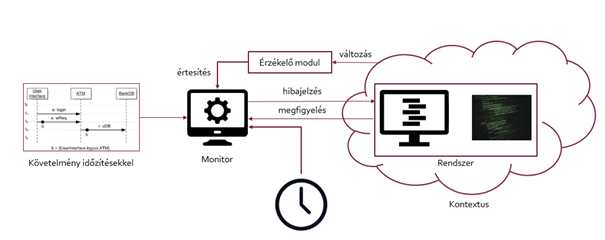
\includegraphics[width=150mm, keepaspectratio]{figures/1abra.png}
    \caption{Kontextusfüggő rendszerek monitorozása időzítési feltételekkel.}
\end{figure}

A scenario alapú monitorozás során a kommunikáció megfigyelésével szeretnénk felismerni a problémákat a rendszerünkben.
A rendszerben lévő objektumok közti interakciókat, üzeneteket fogja megfigyelni a monitor.
A követelményt scenario formájában adjuk meg az üzenet szekvenciák specifikálásához.
Szekvencia diagramok segítségével egyszerűen megadhatunk ilyeneket.
A diagramokat a későbbiekben olyan alakra kell majd hoznunk, hogy abból a monitor létrehozható legyen.

%----------------------------------------------------------------------------
\chapter{Háttérismeretek}\section{A monitorozás alapjai}

Egy monitor feladata az, hogy futási időben egy rendszert megfigyeljen, elemezzen és egy adott követelmény alapján felismerje a rendszer helytelen viselkedését.
Ezt a helytelen viselkedést jelzi a rendszernek, de néhány esetben a rendszer működését is befolyásolhatja.
Ez egy kritikus rendszernél különösen fontos lehet hiszen, egy ilyen rendszernél elvárt, hogy folyamatosan biztonságosan tudjon működni.
Ezen kívül, a monitornak időmérésre is szüksége van, mert a követelmény tartalmazhat időziteseket is.
Az 1.1. ábra bemutatja a monitorozás koncepcióját.

\begin{figure}[!ht]
    \centering
    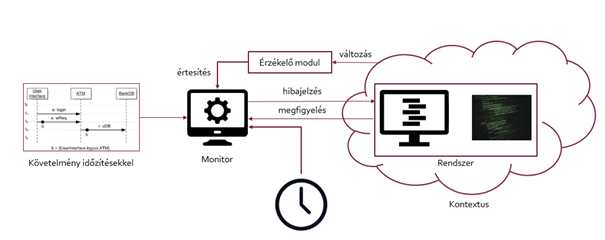
\includegraphics[width=150mm, keepaspectratio]{figures/1abra.png}
    \caption{Kontextusfüggő rendszerek monitorozása időzítési feltételekkel.}
\end{figure}

A scenario alapú monitorozás során a kommunikáció megfigyelésével szeretnénk felismerni a problémákat a rendszerünkben.
A rendszerben lévő objektumok közti interakciókat, üzeneteket fogja megfigyelni a monitor.
A követelményt scenario formájában adjuk meg az üzenet szekvenciák specifikálásához.
Szekvencia diagramok segítségével egyszerűen megadhatunk ilyeneket.
A diagramokat a későbbiekben olyan alakra kell majd hoznunk, hogy abból a monitor létrehozható legyen.

\clearpage\section{Időfüggő viselkedés specifikálására alkalmas formalizmusok áttekintése}
\subsection{MSC - Message Sequence Chart}

Az egyik legelterjedtebb scenario alapú modellezésre használt vizuális formalizmus a
Message Sequence Charts (MSC). A nyelv célja két, vagy több üzeneteket cserélő
objektum között az interakciónak a leírása. A Unified Modelling Language (UML) 2.0
szekvencia diagram leíró részét nagyban inspirálta ez a nyelv.

Az MSC főbb elemei:

\begin{itemize}
    \item MSC head, lifeline és end
    \item Objektum létrehozása
    \item Üzenet csere
    \item Függvényhívás és válasz
    \item Timer-ek
    \item Idő intervallumok
    \item Összetett szerkezetek: alt, opt, parallel, loop (high-MSC)
\end{itemize}

Az összetett szerkezetek a high-MSC (h-MSC) nevű MSC kiterjesztésben találhatók.

Ezzel a nyelvvel már könnyedén lehet a scenarioban lévő üzeneteket specifikálni, és azokat a
rendszer komponenseket, amelyek ezeket az üzeneteket egymásnak küldik.

Az UML és az MSC sokban hasonlítanak, de az alapelveik különbözőek.

MSC-ben a függőleges vonalak („life line”-ok) autonóm entitásokat képviselnek, míg a
szekvencia diagramok esetén ezek egy objektumot reprezentálnak. MSC esetén az
entitásoknak nem szükséges ugyanazon a számítógépen lenniük.

MSC-ben egy átmenet egy aszinkron üzenetet reprezentál, amely két entitás között jött létre,
míg az UML szekvencia diagram leíró nyelvében, egy átmenet egy függvényhívást jelent.

Az MSC-nek sajnos sok hiányossága is tapasztalható. Hiányzik belőle az üzenetek
típusossága. Egy követelmény megfogalmazásakor fontos, hogy meg tudjuk mondani, melyek
az elvárt üzenetek vagy, hogy melyek jelentenek hibát. Az is nagy hiányosságnak számít,
hogy az üzenetekre nem lehetséges megkötéseket megadni. Ez egyben megnehezíti egy
követelmény leírását is.

\subsection{MTL - Metric Temporal Logic}
\subsection{MITL - Metric Interval Temporal Logic}
\subsection{PSC – Property Sequence Chart}
%----------------------------------------------------------------------------
A Message Sequence Chart-nak nagyon sok hiányossága van.
Nem lehet vele megkötéseket definiálni vagy egy üzenetről eldönteni, hogy az egy elvárt vagy nem kívánt üzenet.
Ebből kifolyólag az MSC nem egy alkalmas nyelv arra, hogy az üzenet szekvenciáinkat részletesebben specifikálni tudjuk vele.

\begin{table}[ht]
    \centering % used for centering table
    \begin{tabular}{ |c|c|c| } % centered columns (4 columns)
    \hline
    \textbf{Tulajdonság} & \textbf{MSC} & \textbf{PSC} \\ [0.5ex] % inserts table
    %heading
    \hline % inserts single horizontal line
    \hline
    Nem kivánt üzenet & - & Fail message \\ % inserting body of the table
    \hline
    Elvárt üzenet & - & Required message \\
    \hline
    Sima üzenet & Default message & Regular message \\
    \hline
    Megkötött sorrendezés & - & Strict sequencing \\
    \hline
    Gyenge sorrendezés & Seq & Loose sequencing \\
    \hline
    Üzenet megkötések & - & Constraint \\
    \hline
    Alternatív lehetőségek & h-MSC & Alternative operator \\
    \hline
    Párhuzamos művelet & h-MSC & Parallel operator \\
    \hline
    Ciklus & h-MSC & Loop operator \\
    \hline %inserts single line
    \end{tabular}
    \label{table:nonlin} % is used to refer this table in the text
    \caption{Az MSC összehasonlítása a PSC-vel} % title of Table
\end{table}

A Property Sequence Chart[1] az MSC egy kiterjesztése.
Sok új elemet vezet be ami nincs az MSC-ben, melyek megtekinthetők a 2.1. táblázaton, mint az üzenet típusokat: sima üzenet (e), elvárt üzenet (r) és nem kívánt üzenet (f).
Így specifikálhatjuk, hogy mely üzenetek azok amik helyes viselkedésre utalnak és azok amelyek nem.
Az elvárt üzenetek azok az üzenetek amelyeknek feltétetlen meg kell történiük a rendszer működése során.
Egy sima üzenet nem jelent hibát a monitor szempontjából ha nem történik meg, viszont ha megjelenik, akkor a scenario-ban utána következő üzenetek ellenőrzésére kell áttérni.
Szigorú sorrendezésre is ad megoldást a PSC, ami azt jelenti, hogy megadhatjuk explicit az üzenetek sorrendjét a követelményünkben.
A PSC-ben egy üzenetre megkötést is rakhatunk.
Megadhatjuk, hogy melyek azok az üzenetek amik nem kívántak az üzenetünk előtt vagy után.
A különböző PSC tulajdonságok megtalálhatok a 2.1. ábrán.
A nyelv a következő tulajdonságokat támogatja:

\begin{itemize}
    \item \textit{Sima üzenet (e)}: egy üzenet a scenario-ban, amely ha nem történik meg az a monitor szempontjából nem jelent hibát.
    Viszont ha megjelenik, akkor a scenario-ban utána következő üzenetek ellenőrzésére kell áttérni.
    Egy előfeltételt reprezentál.
    \item \textit{Elvárt üzenet (r)}: egy üzenet amelynek elmaradása hibajelzéshez kell vezessen.
    \item \textit{Nem kívánt üzenet (f)}: amennyiben a monitor egy ilyen üzenetet detektál, akkor hibát jelez.
    \item \textit{Üzenet megkötés (constraint)}: Egy üzenetre lehet megkötést is helyezni.
    Egy megkötés több üzenetet tartalmazhat.
    Két fajta megkötést definiál a nyelv: múlt- és jövőbéli.
    A múltbéli üzenet megkötés esetén, az üzenetünk megtörténte előtt, a megkötésben szereplő üzenetek egyike se történhet meg.
    Jövőbéli megkötés esetén, pedig az üzenetünk megtörténte után nem történhetnek meg a megkötésben szereplő üzenetek.
    \item \textit{Megkötött sorrendezés (strict ordering)}: A PSC az üzenet lefutási sorrendjének a specifikálására is lehetőséget ad.
    Egy „a” üzenet megtörténte után, egy adott „b” üzenetnek kell bekövetkeznie.
    Ha „b” üzenet helyet egy másik üzenet követi az „a” üzenetet, akkor a monitor hibát jelez.
\end{itemize}

A nyelv támogat összetett szerkezeteket is:

\begin{itemize}
    \item \textit{Alt operátor}: az alt operátorral alternatív üzenet szekvenciákat lehet definiálni.
    \item \textit{Par operátor}: a par operátorral meghatározható az üzenet szekvenciák párhuzamos futása.
    \item \textit{Loop operátor}: a loop operátorral megadhatjuk, hogy egy üzenet szekvencia többször is lefuthat egymás után.
\end{itemize}

Egy üzeneten egyszerre megkötés és sorrendezés is lehet.
Az üzenetek típusát az átmenetén lévő karakterrel jelöljük.
Az „e” karakter jelzi, hogy az üzenet sima, az „r” karakter az elvárt üzenetet jelenti, az „f” pedig a nem kívánt üzenetet.
Azt meg kell jegyezni, hogy nem kívánt üzenetekre nem lehet jövőbéli megkötéseket rakni.
Ezen kívül, ha egy üzeneten megkötött sorrendezést alkalmazunk, akkor nem lehet rajta múltbéli megkötés.

A megkötéseket egy ponttal jelöljük, amit az átmeneten helyezünk el.
Ha a pont az átmenet elején van (a feladóhoz közel), akkor az múltbéli megkötést jelöl.
Ha pedig a végén helyezkedik el, akkor a jövőbéli megkötést jelöli.
A megkötésben lévő üzeneteket egy lista formájába lehet megadni ’{’ ’}’ jelek közt, a következő módon: <megkötés neve> = {C1.I1.Cj, ..., Ck.In.Ct}, ahol az üzenetek vesszővel elválasztva, „Feladó.Üzenet.Címzett” formában szerepelnek.
A specifikált megkötés nevét pedig az átmeneten lévő pont alá írjuk.

Az üzenetek megkötött sorrendezésének jelölésénél az objektum „life line” vonalát az érintett átmenetek közt folytonossá változtatjuk

\begin{figure}[!ht]
    \centering
    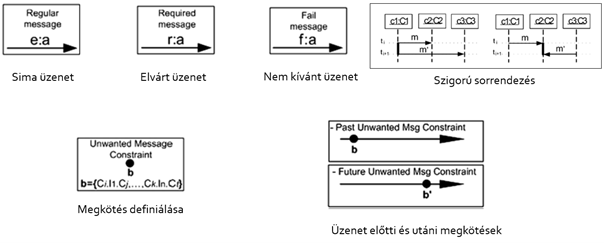
\includegraphics[width=150mm, keepaspectratio]{figures/2abra.png}
    \caption{A PSC különböző elemei[1].}
\end{figure}

Az üzeneteket a következő formában adjuk meg: \textit{Feladó.Üzenet.Címzett}.

\begin{figure}[!ht]
    \centering
    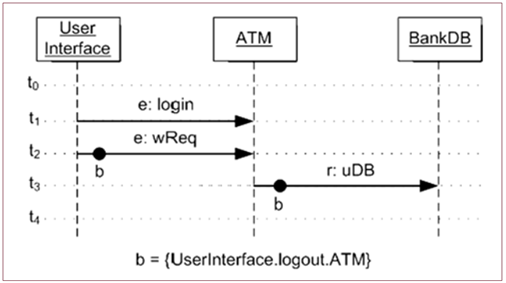
\includegraphics[width=130mm, keepaspectratio]{figures/3abra.png}
    \caption{PSC diagram egy ATM rendszer működésének ellenőrzésére[1].}
\end{figure}
A 2.2. ábrán láthatunk egy példát arra, hogy egy követelményt hogyan lehet definiálni.
Ez a PSC diagram egy ATM rendszer működését figyeli.
Először a felhasználó egy \textit{login} üzenettel bejelentkezik az ATM-be majd egy \textit{wReq} üzenettel egy lekérdezést hajt végre.
Ezen az üzeneten van egy megkötés, az üzenet előtt nem történthet kijelentkezés, \textit{logout}.
Az ATM ezután, ha nem történt \textit{logout} egy elvárt üzenetet küld a Bank adatbázisába.

A scenario-ink specifikálására most már rendelkezésünkre áll egy grafikus nyelv.
A következőkben az lesz a feladatunk, hogy ezeket a diagramokat úgy transzformáljunk, hogy monitor kódot lehessen belőlük készíteni.


%----------------------------------------------------------------------------
\clearpage\section{A TPSC bemutatása}
%----------------------------------------------------------------------------
A TPSC[2] a PSC-nek egy kiterjesztése.
A PSC üzenetekre időzítési feltételeket specifikálhatunk.

\begin{figure}[!ht]
    \centering
    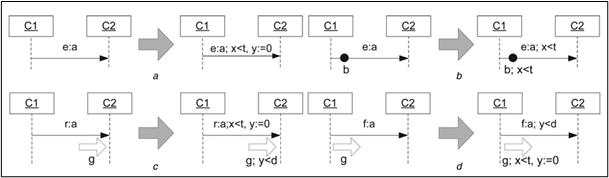
\includegraphics[width=150mm, keepaspectratio]{figures/4abra.png}
    \caption{PSC kiterjesztése időzítési feltételekkel[2].}
\end{figure}

A TPSC óraváltozókat (x, y) használ az időzítéshez.
Ezekre meg lehet adni feltételeket, valamint az óraváltozót lehet nullázni.
A nullázással adott eseménytől (pl. üzenet vételétől) kezdve indul az időzítés, majd rákövetkező események időbeliségét ez alapján lehet ellenőrizni.

A 3.1. ábrán látható, hogy például az \textit{e: a} sima üzenet \textit{e: a; x < t, y := 0} üzenetre bővül.
Elvárjuk, hogy az \textit{a} üzenet \textit{t} idő előtt történjen meg és egy \textit{y} óraváltozót nullázunk.
Az \textit{e: a} üzenet egy sima üzenet, szóval ha nem történik meg a specifikált idő intervallumban az nem jelent hibát.
Viszont \textit{r: a} üzenetnél már elvárt, hogy \textit{t} időn belül megtörténjen. \textit{f: a} üzenet esetében viszont akkor jelez hibát a monitor, ha üzenet megtörtént \textit{t} időn belül.

Egy megkötésre is meg lehet adni időzítési feltételt.
Így megadhatjuk, hogy mennyi ideig nem szabad jönnie a megkötésben szereplő nem kivánt üzenetek egyikének.
Ha a feltételben megadott idő után történik akkor az nem jelent hibát a monitor szempontjából.

% !TeX spellcheck = hu_HU
% !TeX encoding = UTF-8
% !TeX program = xelatex
%----------------------------------------------------------------------------
\clearpage\section{TPSC szcenário alapú automata konstrukció}
%----------------------------------------------------------------------------

A monitorozás alapja, hogy TPSC scenario-kból időzített automatákat (Timed Automata) tudjunk készíteni.
Egy TA állapotokból, elfogadó állapotokból, feltételekből, akciókból és bemenetekkel címkézett állapotátmenetekből áll.
Akkor fogad el egy bemenet sorozatot, ha ennek során elérünk az automata végállapotába.
Ha elfogadó állapotot érünk el, akkor az a monitor szempontjából hibát jelent.
Az alapelv az az, hogy minden TPSC elemhez tartozik egy minta automata (pattern) ami leírja a szemantikáját.
Például a 4.1. és 4.2. ábrákon láthatóak a különböző PSC üzenetekhez tartozó minták.

\begin{figure}[!ht]
    \centering
    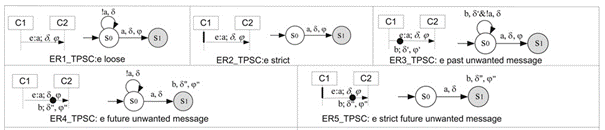
\includegraphics[width=150mm, keepaspectratio]{figures/5abra.png}
    \caption{Sima üzenetekhez tartozó minták[2].}
\end{figure}

\begin{figure}[!ht]
    \centering
    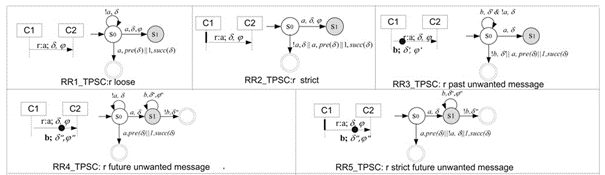
\includegraphics[width=150mm, keepaspectratio]{figures/6abra.png}
    \caption{Elvárt üzenetekhez tartozó minták[2].}
\end{figure}

A minta automatánkban található szürke állapotok reprezentálják a végállapotokat.
A megkötéseket az automatáknál egy átmenettel definiáljuk ami a nem kívánt üzenetek negáltjainak az ÉS kapcsolata.
Például az 4.1. ábrán lévő 3. automata mintán látható „b, $\delta ’\&!a, \delta$” címkéjű hurokélen, a „b” címke minden olyan üzenetnek felel meg, amelyek nincsenek a nem kivánt üzenetek halmazában.
A címke teljes jelentése az, hogy ha $\delta$’ időn belül nem jött nem kivánt üzenet és $\delta$ időn belül nem az „a” üzenet jött akkor maradjunk az s0 állapotban.
Ezekből az automata részekből lesznek meghatározott illesztési szabályokkal a scenario-hoz tartozó teljes időzített automaták.
Ennek az az alapelve, hogy a scenario-n végig menve az előző minta végállapotát a következő minta kezdőállapotával kell egyesíteni.
Ezt a folyamatot mutatják be a 4.3., 4.4. és 4.5. ábrák.

\begin{figure}[!ht]
    \centering
    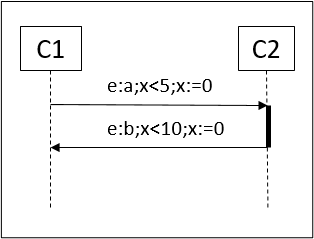
\includegraphics[width=60mm, keepaspectratio]{figures/7abra.png}
    \caption{TPSC részlet.}
\end{figure}

\begin{figure}[!ht]
    \centering
    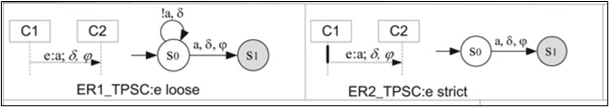
\includegraphics[width=150mm, keepaspectratio]{figures/8abra.png}
    \caption{Alkalmazott automata minták.}
\end{figure}

\begin{figure}[!ht]
    \centering
    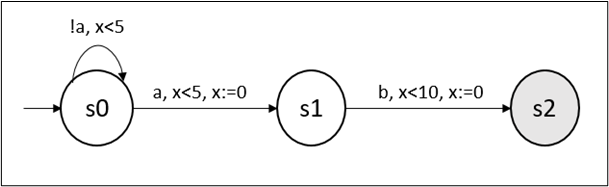
\includegraphics[width=130mm, keepaspectratio]{figures/9abra.png}
    \caption{Az összeállított automata.}
\end{figure}

A monitor szempontjából az automata akkor jelez hibás működést ha elfogadó állapotba kerül.
Ilyenkor a követelmény már nem teljesíthető.
Ha az automata egy sima állapotban van, akkor az helyes működést jelent viszont a követelmény még ekkor sem teljesült.
A követelmény akkor teljesül amikor az automata a végső (FINAL) állapotba kerül és nem érkezik további amely elmozditaná őt onnan.
\section{A felhasznált technológiák}
\subsection{Eclipse}

Az \textit{Eclipse} \cite{Eclipse} egy nyílt forráskódú, platformfüggetlen keretrendszer.
Első sorban fejlesztői környezetként használják.
A keretrendszert tovább lehet bővíteni mindenféle \textit{plugin} telepítésével, így például modellezésre is alkalmas lehet.
A projektem során használt \textit{Eclipse} \textit{plugin}-ok:

\begin{itemize}
    \item \textit{Xtext} \cite{Xtext}
    \item \textit{Xtend} \cite{Xtend}
    \item \textit{Sirius} \cite{Sirius}
\end{itemize}

A munkafolyamat egy \textit{workspace}-en belül történik, ahol a fejlesztő létrehozhatja a saját projektjeit.
Több \textit{workspace}-t is létre lehet hozni és azok között váltani.

Különböző fajta projekteknek különböző nézetei lehetnek.
Például egy modellező projektnek van külön modell nézete az eszközön belül vagy egy \textit{Java} projektnek \textit{Java} nézete.
A nézetek az eszközön megjelenített szövegszerkesztő, fájlkezelő vagy egyéb funkció elhelyezéséért, megjelenítéséért felelnek.

\subsection{Xtext}

Az \textit{Xtext} \cite{Xtext} \textit{Eclipse} \textit{plugin}-nel programozási és \textit{domain} specifikus nyelveket lehet fejleszteni.
A nyelvünk elemeit és szabályait egy nyelvtan segítségével definiálhatjuk.
Az \textit{Xtext} keretrendszer több eszközt nyújt a nyelvünkhöz, például egy \textit{parser}-t, egy fordítót és egy szerkesztőt.
A \textit{plugin} még egy \textit{Xtend} alapú kódgenerátort is generál a nyelvünkhöz, amivel a nyelvünkhöz tetszőleges kódot tudunk generálni.

\begin{lstlisting}[language=java, frame=single, float=ht!, caption={Xtext nyelvtan elemei.},captionpos=b, label=XtextGrammar]
Scenario:
	'scenario' name=ID '{'
	scenariocontents+=ScenarioContent*
	'}'
;

ScenarioContent:
	alt+=Alt | message+=Message | par+=Par | loop+=Loop | paramConstraint+=ParameterConstraint

;

Message:
	LooseMessage | StrictMessage | PastMessage | FutureMessage | StrictFutureMessage
	| RequiredLooseMessage | RequiredStrictMessage | RequiredPastMessage | RequiredFutureMessage | RequiredStrictFutureMessage
	| FailMessage | FailStrictMessage | FailPastMessage
;

LooseMessage:
	'message' name=ID '(' (params+=Params | constantparams+=ConstantParams) ')'
	sender=[Object] '->' receiver=[Object]
	('clockConstraint' '{' cConstraint=ClockConstraintExpression '}')? 
	(resetclock=ResetClock)? ';'
;
\end{lstlisting}

A \ref{XtextGrammar}-es kódrészlet az \textit{Xtext} nyelvtan elemeit mutatja be.
Egy nyelvtani szabályt egy tetszőleges név megadásával hozhatunk létre, a szabályunkat pedig a név után lévő ":" és ";" közzé írhatjuk.
Idézőjelek közé írhatjuk a nyelvünkhöz tartozó kulcsszavakat, például \textit{'scenario'} vagy idézőjelek között kapcsos zárójel.
Ilyen kulcsszavak megadásával jól tudjuk formázni a nyelvtani szabályunkat.
Attribútumok megadásával tudjuk tárolni a nyelvi elemünk értékeit, változóit, például a \textit{name} attribútum egy \textit{ID} elemet tárol, ami egy azonosítónak felel meg.
Egy attribútumba több elemet is rakhatunk lista szerűen.
Ezt a \textit{*} karakterrel adhatjuk meg, például \textit{scenariocontents+=ScenarioContent*}, ahol a \textit{scenariocontents} több \textit{ScenarioContent}-beli elemet tárol.
A \textit{+=} karakterrel pakolhatjuk az új \textit{ScenarioContent}-jeinket a \textit{scenariocontents} tömbbe.

A nyelvtanunkban megadhatunk elágazó szabályokat is a "|" karakterrel.
Ilyen szabály például a \textit{Message}.
Továbbá hivatkozhatunk már létrehozott nyelvi elemekre is a szabályunkban a "[]" szintakszissal.
Például a \textit{LooseMessage} \textit{sender} attribútuma egy már létrehozott \textit{Object} elemre hivatkozik.

A "?" karakter opcionális nyelvi elemek megadására szolgál.

Fordítás után a nyelvi elemeinkből \textit{Xtend} és \textit{Java} osztályok generálódnak.

\subsection{Xtend}

Az \textit{Xtend} \cite{Xtend} egy magasszintű programozási nyelv, amely a \textit{Java Virtual Machine} platformot használja.
Szintaktikailag és szemantikailag nagyon hasonlít a \textit{Java} nyelvhez, mondhatni a \textit{Java} kibővítése.
Az \textit{Xtend} fordító a létrehozott osztályokból \textit{Java} osztályokat generál.
Így akár könnyedén ki tudjuk szervezni a projektünket egy \textit{.jar} fájlba.

Egy nagyon hasznos funkciója az \textit{Xtend}-nek a \textit{template}, amely segítségével sablonokat hozhatunk létre a függvényeken belül, így megkönnyítve a kódgenerálást.
Így tudunk hivatkozni az \textit{Xtext} nyelvi elemeinkre függvény paramétereken keresztül és egyedi kódgenerátort fejleszteni a nyelvünkhöz.
A sablon függvényen belül a "«»" karaktereket használva tudunk hivatkozni az \textit{Xtext} nyelvi elemeinkre.

\begin{lstlisting}[language=java, frame=single, float=ht!, caption={Xtend template.},captionpos=b, label=XtendTemplate]
def compile(Scenario scenario)'''
	«FOR sc : scenario.scenariocontents»
		«FOR m : sc.message»
			«generateMessage(m)»
			a.collapse(b);
		«ENDFOR»
	«ENDFOR»
'''
\end{lstlisting}

A \ref{XtendTemplate} ábra egy \textit{Xtend} sablon függvényt mutat be.
A "«»" karaktereket használva hivatkozhatunk a paraméterben átadott \textit{Xtext} nyelvbeli objektum attribútumaira.
Itt például a \textit{Scenario} \textit{scenariocontents} tömbjén megyünk végig.

\subsection{Sirius}

A \textit{Sirius} \cite{Sirius} eszköz segítségével létrehozhatunk saját grafikus modellező alkalmazásainkat.
Egy szerkesztő környezetet alkothatunk, amivel a modellünk elemeit hozhatjuk létre, vagy szerkeszthetjük grafikusan.
A \textit{plugin} az \textit{Entity Modelling Framework} \cite{EMF} keretrendszert használja a modellek feldolgozásához és ilyen \textit{EMF} modelleket jelenít meg.
Ehhez az \textit{EMF} modellünk összes eleméhez meg kell adnunk egy megjelenítést.

Elkészíthetjük saját egyedi szerkesztőnket, de választhatunk a \textit{Sirius} által nyújtott szerkesztőkből is:
\begin{itemize}
	\item Diagram
	\item Szekvencia diagram
	\item Táblázat
\end{itemize}

Az egyes modell elemeinkhez tartozó grafikus megjelenítést egy \textit{viewpoint} létrehozásával tudjuk megtenni.
A \ref{sirius_viewpoint} ábrán látható egy példa \textit{viewpoint}.
A \textit{viewpoint}-hoz hozzá fűzhetünk egy \textit{representation}-t amely a konkrét megjelenítésünket tartalmazza.
Itt adhatjuk meg, hogy egyes modell elemeink milyen formában jelenjenek meg.

\begin{figure}[!ht]
    \centering
    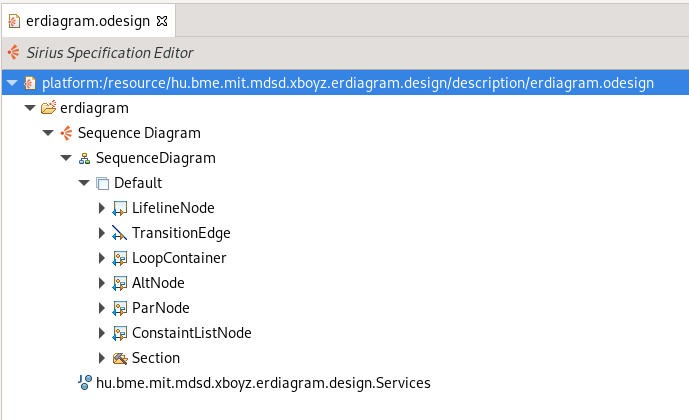
\includegraphics[width=150mm, keepaspectratio]{figures/sirius_viewpoint.png}
    \caption{\textit{Sirius} alkalmazáshoz tartozó \textit{viewpoint}.}
    \label{sirius_viewpoint}
\end{figure}

Emellett alkalmazhatunk feltételes megjelenítést is adott típusú modellelemünkre, ha az adott tulajdonságban eltér a többi elemtől.
%----------------------------------------------------------------------------
\chapter{Monitor generálás terv és feladat megfogalmazása}
%----------------------------------------------------------------------------

\begin{figure}[!ht]
    \centering
    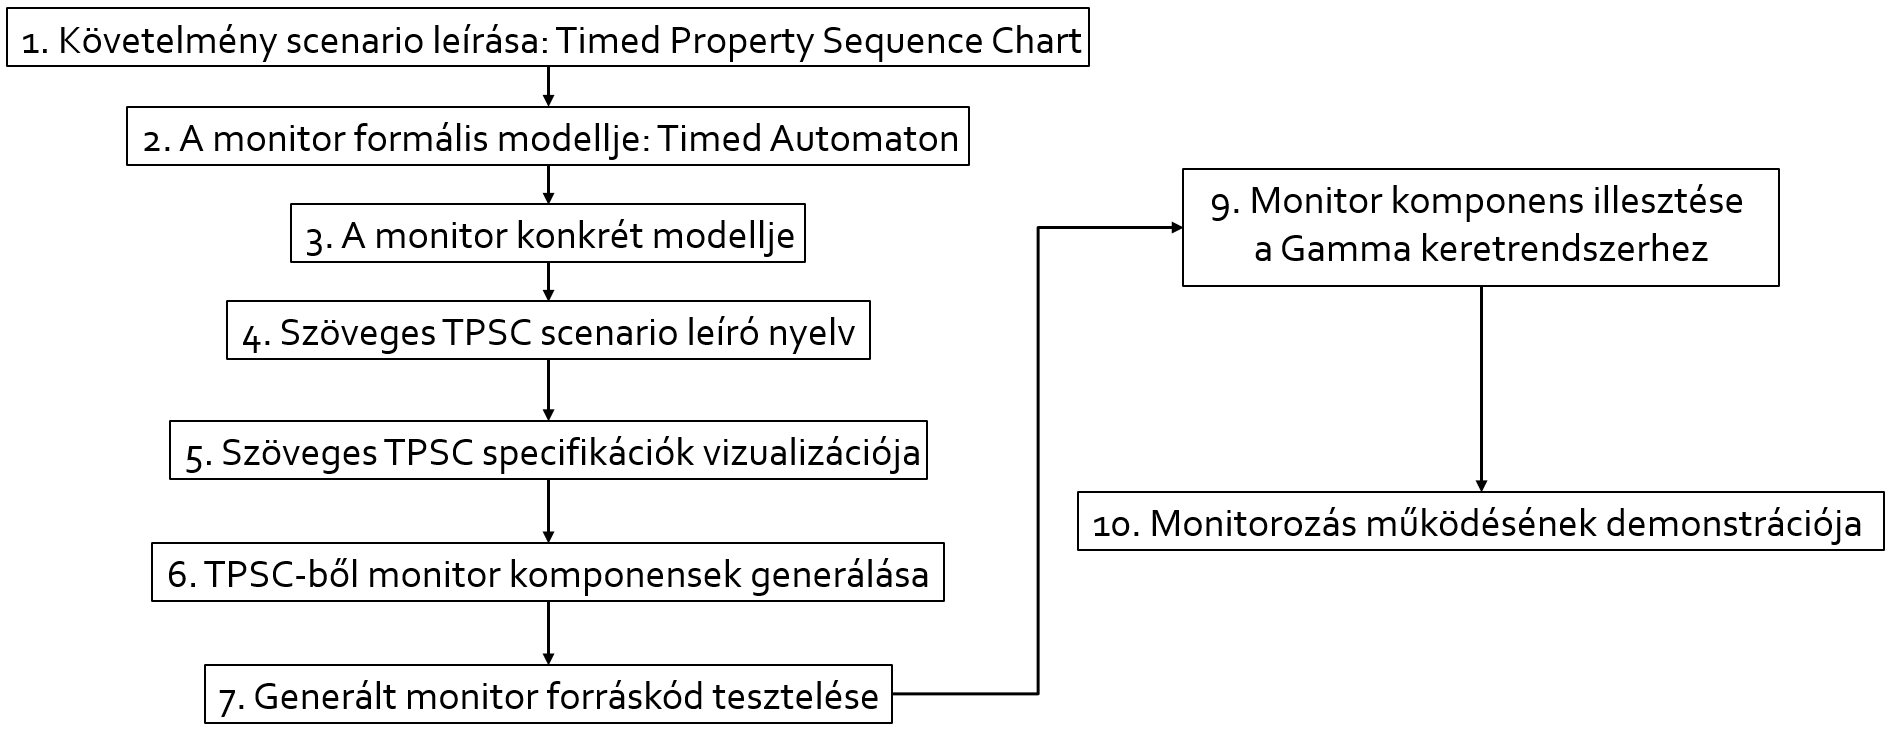
\includegraphics[width=150mm, keepaspectratio]{figures/generation_plan.png}
    \caption{Monitor generátor kibővítése.}
\end{figure}

A cél az, hogy a „Monitor komponensek generálása kontextusfüggő viselkedés ellenőrzése” című szakdolgozatom során elkészített monitor komponens generátort kibővíteni úgy, hogy támogassa időzítési feltételek megadását.
A monitor generálás terve látható a 5.1. ábrán.
Az Önálló laboratórium keretében az volt a feladatom, hogy a szakdolgozat során definiált szöveges PSC diagram leíró nyelvet kibővitsük a TPSC elemeivel.
Ezután az automata generátort kell úgy kibővíteni, hogy a TPSC diagramokból tudjon TA automatákat generálni.
Egy monitor forráskód generátor pedig az automata alapján elkészítheti a monitor forráskódját.

A szöveges TPSC scenario leírásához el kell készítenünk a diagram vizualizációját, hogy grafikusan megtekinthessük a definiál scenario-t.
A következő a generált monitor forráskód tesztelése, majd ezután ezt illeszük a Gamma keretrendszerhez.
Ezzel az a célunk, hogy elosztott komponens alapú rendszerek szimulációja közben monitorozható legyen a TPSC üzenet szekvencia specifikáció teljesülése illetve az ebben rögzített tulajdonságok megsértése

A Diplomatervezés 1 tárgy keretében a tervnek a negyedik, hatodik és hetedik részeivel foglalkoztam.
%----------------------------------------------------------------------------
\chapter{Szöveges PSC leíró nyelv kibővítése}
%----------------------------------------------------------------------------

A szakdolgozatom során készített szöveges \textit{PSC} leíró nyelvet \cite{Bakai} az \textit{Xtext} technológia segítségével definiáltam.
A nyelv fő elemei:
\begin{itemize}
    \item objektumok (az üzenetekkel kommunikáló rendszerkomponensek)
    \item üzenetek
    \item megkötések
    \item szcenárió
    \item \textit{alt} operátor
    \item \textit{loop} operátor
    \item \textit{par} operátor
\end{itemize}

A nyelvben egy objektumot az „\textit{object}” kulcsszóval lehet bevezetni.
Meg kell adni az objektum típusát és a nevét, ezután a definíciót egy ’;’-vel lehet lezárni.
Megkötések specifikálásához a „\textit{constraint}” kulcsszót kell használni.
Elég csupán a megkötés nevét megadni és '\{' '\}' jelek közt, a megkötéshez tartozó üzeneteket.

Egy sima üzenet megadásához a „\textit{message}” kulcsszó szükséges.
A „\textit{message}” kulcsszó előtt lévő „\textit{fail}” vagy „\textit{required}” kulcssavakkal adhatunk meg nem kívánt vagy elvárt üzeneteket.
A „\textit{strict}” kulcsszóval adhatjuk meg, hogy az üzenet sorrendje megkötött.
Az üzenet küldőjét és fogadóját „\textit{<küldő> $\,\to\,$ <fogadó>}” formában jelezzük.
Múltbeli vagy jövőbeli megkötéseket a „\textit{pastConstraint}" vagy „\textit{futureConstraint}" kulcsszavakkal adhatunk meg.
A kulcsszó után, '\{' '\}' jelek közt adhatjuk meg, hogy melyik előzőleg definiált megkötést helyezzük el az üzeneten.
Egy üzenet definíció végére szükséges ’;’-t tenni, így elválasztjuk a többi üzenettől.

A nyelvet két új elemmel bővítettem ki:
\begin{itemize}
    \item időzített feltétel
    \item óraváltozó nullázása
\end{itemize}
Az új nyelvi elemek bevezetéséhez az eredeti üzenet leíró \textit{Xtext} szabályt (\textit{Message}) kellett kibővítenem.
A kibővített nyelvtani szabályt a \ref{minotor_message} kódrészlet tartalmazza.
Az eredeti nyelvtani szabályt a \ref{minotor_message_original} kódrészlet tartalmazza.
Bevezettem egy új \textit{clockConstraint} kulcsszót, amellyel egy időzítési feltételt lehet megadni.
Ezt a \textit{cConstraint} változóban tárolom.
A \textit{resetClock} attribútum tárolja a visszaállítandó óraváltozó nevét.
A teljes nyelvtan definíció megtekinthető a \textit{Függelékben} (\ref{xtext_tpsc_grammar}).

\begin{lstlisting}[language=java, frame=single, float=ht!, caption={Eredeti \textit{Message} nyelvtani szabály \cite{Bakai}.},captionpos=b,label=minotor_message_original]
Message:
    'message' name=Name (required?='required')? (fail?='fail')? (strict?='strict')?
    sender=[Object] '->' receiver=[Object]
    (past?='past')? (future?='future')? (constraint?='constraint')?
    ('{')? (c=[Constraint])? ('}')? ';'

;
\end{lstlisting}

\begin{lstlisting}[language=java, frame=single, float=ht!, caption={Kibővített \textit{Message} nyelvtani szabály.},captionpos=b,label=minotor_message]
Message:
	LooseMessage | StrictMessage | PastMessage | FutureMessage | StrictFutureMessage
	| RequiredLooseMessage | RequiredStrictMessage | RequiredPastMessage | RequiredFutureMessage | RequiredStrictFutureMessage
	| FailMessage | FailStrictMessage | FailPastMessage
;

LooseMessage:
	'message' name=ID '(' (params+=Params | constantparams+=ConstantParams) ')'
	sender=[Object] '->' receiver=[Object]
	('clockConstraint' '{' cConstraint=ClockConstraintExpression '}')?
	(resetclock=ResetClock)? ';'
;
\end{lstlisting}

\begin{figure}[!ht]
    \centering
    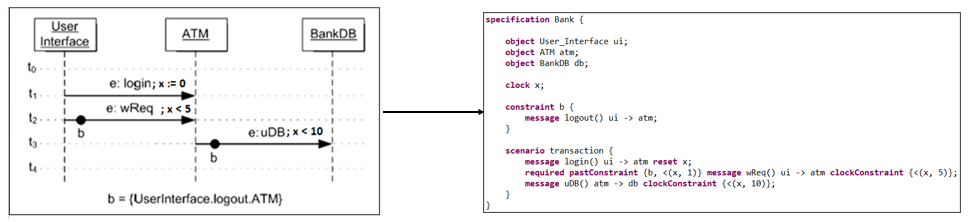
\includegraphics[width=150mm, keepaspectratio]{figures/11abra.png}
    \caption{\textit{TPSC} diagramból szöveges leírás az \textit{Xtext} nyelv használatával.}
    \label{xtext_language_example}
\end{figure}

A \ref{xtext_language_example} ábrán látható, hogy egy \textit{TPSC} diagramot hogyan tudunk leírni a nyelvünk segítségével.
Definiálhatjuk a diagramban szereplő objektumokat, a megkötéseket, amelyeket használni fogunk és végül, hogy milyen üzenetek vannak a követelményünkben.

\begin{figure}[!ht]
    \centering
    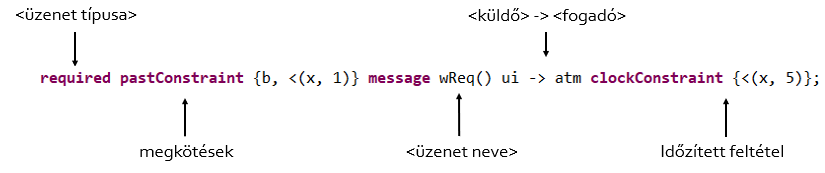
\includegraphics[width=150mm, keepaspectratio]{figures/12abra.png}
    \caption{Egy \textit{TPSC} üzenet felépítése a definiált \textit{Xtext} nyelvben.}
    \label{xtext_message}
\end{figure}

A \ref{xtext_message} ábrán megjelenik a \textit{clockConstraint} kulcsszó, amely egy időzítési feltétel megadására szolgál.
A kulcsszó után kapcsos zárójelek közt megadható a feltétel.
Egy időzítési feltételt egy adott óraváltozóra adhatunk meg.
Négy operátort definiál ehhez a nyelv:
\begin{itemize}
    \item < (kisebb)
    \item > (nagyobb)
    \item <= (kisebb egyenlő)
    \item >= (nagyobb egyenlő)
\end{itemize}
Az operátor után ’(’ ’)’ jelek között adható meg az óraváltozó, majd utána az érték.
Például a \textit{<(x, 5)} kifejezés azt jelenti, hogy az \textit{x} óraváltozóban lévő időértéknek kisebbnek kell lennie öt időegységnél.

Időzítési feltételt egy megkötésre is megadhatunk, '\{' '\}' jelek között, ’,’-vel elválasztva a megkötés után.
A \textit{reset} kulcsszó az óraváltozó nullázására szolgál.
%----------------------------------------------------------------------------
\chapter{Monitor forráskód generálás}\section{Időzített automata generátor}
%----------------------------------------------------------------------------

%----------------------------------------------------------------------------
\subsection{Az automata generátor célja}
%----------------------------------------------------------------------------

Az \textit{önálló laboratórium} során elkészített automata generátort kibővítettem úgy, hogy támogassa a \textit{TPSC} elemekhez tartozó automata minták generálását. Bemenetként egy \textit{TPSC} szcenárió szöveges leírását kapja meg amiből a minta alapú módszerrel generál egy \textit{TA} automatát.

A \ref{tpsc_alt} és \ref{tpsc_alt_nc} kódrészleteken látható, hogy a monitor generátor támogatja az összetett operátorokat tartalmazó \textit{TPSC}-khez tartozó \textit{TA}-k generálását is.
A \ref{tpsc_alt_nc} kódrészlet a generált automata "\textit{never claim}" leírását tartalmazza.
A \textit{Never claim} a \textit{Promela} nyelv része, ezzel egy rendszer viselkedését lehet definiálni.
Továbbá a generátor képes az üzenet paraméterek kezelésére.
Például az \textit{alt} operátor feltételét képes feldolgozni és azt elhelyezni a generált automata megfelelő élén.

\begin{lstlisting}[language=java,frame=single, float=h!, caption={Alt operátort tartalmazó szcenárió.},captionpos=b,label=tpsc_alt]
specification Bank {

	object UserInterface ui;
	object ATM atm;
	object BankDB db;

	bool success = true;

	constraint b {
		message logout() ui->atm;
	}

	scenario transaction {
		message login(success) ui->atm;

		alt (equals(success, true)) {
			message wReq() ui->atm;
			message uDB() atm->db;
		} (equals(success, false)) {
			message loginUnsuccessful() ui->atm;
			message lockMachine() required atm->ui;
		}
	}
}
\end{lstlisting}

\begin{lstlisting}[language=java,frame=single, float=h!, caption={Alt operátort tartalmazó szcenárió never claim leírása.},captionpos=b,label=tpsc_alt_nc]
bool success = true;

never{ /*transactionMonitor*/
T0_init:
 if
 :: (!(ui.login(success).atm)) -> goto T0_init
 :: (ui.login(success).atm) -> goto T0_q1
 fi;
T0_q1:
 if
 :: (epsilon) -> goto T0_qinit0
 fi;
T0_qinit0:
 if
 :: (epsilon; success == true) -> goto T0_q2
 :: (epsilon; success == false) -> goto T0_q5
 fi;
T0_qfinal1:
 if
 fi;
T0_q2:
 if
 :: (!(ui.wReq().atm)) -> goto T0_q2
 :: (ui.wReq().atm) -> goto T0_q3
 fi;
T0_q3:
 if
 :: (!(atm.uDB().db)) -> goto T0_q3
 :: (atm.uDB().db) -> goto T0_q4
 fi;
T0_q4:
 if
 :: (epsilon) -> goto T0_qfinal1
 fi;
T0_q5:
 if
 :: (!(ui.loginUnsuccessful().atm)) -> goto T0_q5
 :: (ui.loginUnsuccessful().atm) -> goto T0_q6
 fi;
T0_q6:
 if
 :: (!(atm.lockMachine().ui)) -> goto T0_q6
 :: (!(atm.lockMachine().ui)) -> goto accept_q7
 :: (atm.lockMachine().ui) -> goto T0_q8
 fi;
accept_q7:
 if
 fi;
T0_q8:
 if
 :: (epsilon) -> goto T0_qfinal1
 fi;
}
\end{lstlisting}

%----------------------------------------------------------------------------
\subsection{Az automata generátor megvalósítása}
%----------------------------------------------------------------------------
A generátorhoz az \textit{Xtend} technológiát használtam.
Minden egyes \textit{TPSC} üzenethez legenerálja a hozzá tartozó minta automatát, majd elvégzi azok összecsatolását.

Az időzített automaták generálásához egy adatstruktúrát definiáltam, amely a következő \textit{Java} osztályokból és interfészekből áll:
\begin{itemize}
    \item AltExpressionInterface
    \item Automaton
    \item BasicTransition
    \item ClockConstraint
    \item ClockExpressionInterface
    \item Constraint
    \item EpsilonTransition
    \item OperatorFunctions
    \item State
    \item StateType
    \item Transition
    \item UnwantedConstraint
    \item WantedConstraint
\end{itemize}

Az automatában lévő állapotok implementációja a \textit{State} osztályban található.
Két attribútuma van:
\begin{itemize}
	\item id(\textit{String}): a címkéje tárolására
	\item type(\textit{StateType}): az állapot típusa
\end{itemize}

Az állapot típusának a megadására a \textit{StateType} enum osztályt definiáltam.
Az enum a következő értékeket veheti fel:
\begin{itemize}
	\item NORMAL
	\item ACCEPT
	\item FINAL
\end{itemize}

Az átmenetek implementációjáért felelős osztály a \textit{Transition}.
Három tag változója van:
\begin{itemize}
	\item id(\textit{String}): az üzenet
	\item sender(\textit{State}): a feladó állapot
	\item receiver(\textit{State}): a fogadó állapot
\end{itemize}

Az időzített automata implementációja az \textit{Automaton} osztályban található.
Itt tároljuk az automatában lévő állapotokat és a köztük lévő átmeneteket egy-egy listában.
Az \textit{Automaton} osztály \textit{addState(State)} és \textit{addTransition(Transition)} függvényeivel lehet új állapotot és átmenetet hozzáadni az automatához, a \textit{collapse(Automaton)} függvényével pedig két automatát egyesíteni.
Ezt a függvényt használtam az implementációban a minta automaták egyesítésére.
Ezen kívül az osztálynak van egy \textit{merge(ArrayList<Automaton>)} függvénye.
Ez a függvény a minta automata ágak egyesítésére szolgál.

A \textit{Specification} osztály feladata, hogy összeállítsa a szöveges leírásban specifikált \textit{TPSC} szcenárióhoz tartozó időzített automatát.
Ezt követően az automata \textit{Never Claim} leírását egy \textit{.txt} kiterjesztésű fájlba írja.

%----------------------------------------------------------------------------
\subsection{Mintapélda}
%----------------------------------------------------------------------------

\begin{figure}[h!]
    \centering
    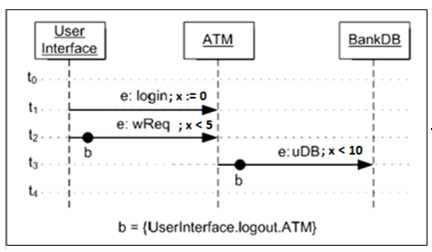
\includegraphics[width=130mm, keepaspectratio]{figures/14abra.png}
    \caption{Példa TPSC diagram.}
	\label{tpsc_example_diagram}
\end{figure}

\begin{lstlisting}[language=java,frame=single, float=h!, caption={TPSC scenario szöveges leírása.},captionpos=b,label=tpsc_example_text]
specification Bank {

	object User_Interface ui;
	object ATM atm;
	object BankDB db;

	clock x;

	constraint b {
		message logout() ui -> atm;
	}

	scenario transaction {
		message login() ui -> atm reset x;
		required pastConstraint {b, <(x, 1)} message wReq() ui -> atm clockConstraint {<(x, 5)};
		message uDB() atm -> db clockConstraint {<(x, 10)};
	}
}
\end{lstlisting}

\begin{lstlisting}[language=java,frame=single, float=h!, caption={Generált időzített automata never claim formátumban.},captionpos=b,label=tpsc_example_nc]
never{ /*transactionMonitor*/
T0_init:
 if
 :: (!(ui.login().atm); ) -> goto T0_init
 :: (ui.login().atm; x = 0) -> goto T0_q1
 fi;
T0_q1:
 if
 :: (!(ui.wReq().atm); x < 5 & !(ui.logout().atm); x < 1)) -> goto T0_q1
 :: (ui.wReq().atm; x < 5) -> goto T0_q3
 :: ((!(!(ui.logout().atm); x < 1); x < 5) || (ui.wReq().atm; )) || (1, x >= 5))) -> goto accept_q2
 fi;
accept_q2:
 if
 fi;
T0_q3:
 if
 :: (!(atm.uDB().db); x < 10;) -> goto T0_q3
 :: (atm.uDB().db; x < 10;) -> goto T0_q4
 fi;
T0_q4:
 if
 fi;
}
\end{lstlisting}

A \ref{tpsc_example_text}, \ref{tpsc_example_nc} kódrészleteken és \ref{tpsc_example_diagram} ábrán látható, hogy a generátor milyen időzített automatát generál a megadott \textit{TPSC} szcenárió-ból.
%----------------------------------------------------------------------------
\section{Monitor forráskód generátor}
%----------------------------------------------------------------------------

%----------------------------------------------------------------------------
\subsection{A monitor interfészei}
%----------------------------------------------------------------------------

\begin{figure}[h!]
    \centering
    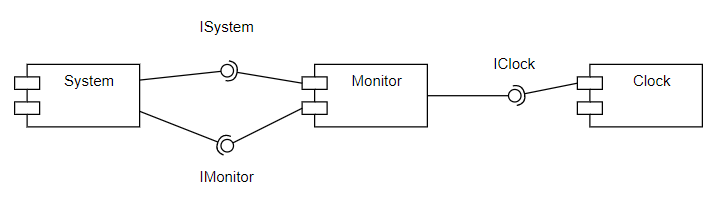
\includegraphics[width=130mm, keepaspectratio]{figures/monitor_architecture.png}
    \caption{Monitor architektúra diagram.}
	\label{monitor_architecture}
\end{figure}

A \ref{monitor_architecture} ábrán látható a megfigyelt rendszer és monitor architektúra diagramja.
A monitorozás alatt lévő rendszer egy \textit{IMonitor} interfészen keresztül kommunikál a monitorral.
Az interfész \textit{Java} implementációja a \ref{IMonitor_interface} kódrészleten tekinthető meg.
A monitor azt vizsgálja, hogy a rendszer a szcenárió szerint viselkedik-e.
A monitornak a következő interfészt kell megvalósítania:
\begin{itemize}
    \item \textit{update()}: ezzel a függvénnyel lehet továbbítani a rendszer üzeneteit a monitor számára.
	Bemenetként az üzenet feladóját, címzettjét, nevét és paramétereit kapja.
	A monitor frissíti a belső automatájának állapotát.
    \item \textit{goodStateReached()}: a rendszer ezen a függvényen keresztül kérdezi le a monitortól, hogy jó állapotban van-e a követelmény szempontjából, azaz nem történt-e hiba.
    Visszatérési értéke egy \textit{boolean} érték.
    \item \textit{requirementSatisfied()}: a rendszer ezzel a függvénnyel kérdezheti le, hogy megfelel-e a követelménynek.
    Visszatérési értéke egy \textit{boolean} érték.
	\item \textit{errorDetected()}: ez a függvény tartalmazza a hibaelhárító funkcionalitás implementációját.
	A rendszer ezt a függvényt használhatja hibaelhárításra hiba detektálás esetén.
	Bemenetként azt az üzenetet kapja meg, amely hatására előjött a hiba az \textit{update()} függvényhez hasonlóan.
    \item \textit{noMoreMessages()}: a rendszer ezen a függvényen keresztül jelzi a monitornak a kommunikáció végét.
\end{itemize}

Az üzenetek megfigyeléséhez szükséges segédfüggvényeket a kommunikációs infrastruktúrához kézzel kell megírni.
Ezek a monitort az \textit{update()} függvényen keresztül hívják.

\begin{lstlisting}[language=java,frame=single, float=h!, caption={Monitor interfész \textit{Java} implementációja.},captionpos=b,label=IMonitor_interface]
public interface IMonitor {
	public boolean goodStateReached();
	public void update(String sender, String receiver, String messageType, Map<String, Object> parameters);
	public boolean requirementSatisfied();
	public void errorDetected(String sender, String receiver, String messageType, Map<String, Object> parameters);
	public void noMoreMessages();
}
\end{lstlisting}

Az időzítési feltételek kiértékelése érdekében a monitornak szüksége van egy időzítő komponensre.
Az időzítő komponenshez tartozik egy időzítő interfész amin keresztül elérhető a komponens.
Ezen az interfészen keresztül lehet az óraváltozókat lekérdezni vagy nullázni.
Két függvénye van:

\begin{itemize}
    \item \textit{getClock(String clock)}: óraváltozó lekérdezése név alapján.
    \item \textit{resetClock(String clock)}: óraváltozó nullázása név alapján.
\end{itemize}

\begin{lstlisting}[language=java,frame=single, float=h!, caption={Időzitő interfész \textit{Java} implementációja.},captionpos=b,label=IClock_interface]
public interface IClock {
	public long getClock(String clock);
	public void resetClock(String clock);
}
\end{lstlisting}

Az \ref{IClock_interface} kódrészlet tartalmazza az időzítő interfész implementációját, az \textit{IClock} \textit{Java} interfészt.

A monitor az \textit{ISystem} interfészen keresztül tud a rendszernek üzeneteket küldeni a megfigyelt viselkedésről.
Ezt az interfészt a monitorozott rendszer valósítja meg.
Három függvénye van:
\begin{itemize}
	\item \textit{receiveMonitorStatus()}: a monitor jelzi a rendszer felé a követelmény alapján az aktuális státuszt.
	Bemenetként a monitor által küldött üzenetet kapja meg.
	\item \textit{receiveMonitorError()}: a monitor jelzi a rendszer felé, ha hibát detektált.
	Bemenetként két üzenetet kap: a hibát okozó üzenetet és az utolsó üzenetet, amikor még a rendszer jó állapotban volt a követelmény szempontjából.
	\item \textit{receiveMonitorSuccess()}: a monitor jelzi a rendszer felé, ha teljesült a követelmény.
\end{itemize}

\begin{lstlisting}[language=java,frame=single, float=h!, caption={Rendszer interfész \textit{Java} implementációja.},captionpos=b, label=ISystem_interface]
public interface ISystem {
	public void receiveMonitorStatus(String message);
	public void receiveMonitorError(String actualMessage, String lastAcceptedMessage);
	public void receiveMonitorSuccess();
}
\end{lstlisting}

Az \ref{ISystem_interface}-es kódrészlet tartalmazza az \textit{ISystem} \textit{Java} interfészt.

%----------------------------------------------------------------------------
\subsection{A monitor forráskód megvalósítása}
%----------------------------------------------------------------------------
A generált forráskód struktúrája egy statikus és egy generált dinamikus részből áll.
A statikus részbe az időzített automata \textit{Java} osztályai kerülnek:
\begin{itemize}
    \item \textit{State}: egy állapotot leíró osztály
    \item \textit{Transition}: egy átmenetet reprezentáló osztály
    \item \textit{Automaton}: egy automatát megvalósító osztály
\end{itemize}
Ezek segédosztályok, amelyek a generált automata reprezentálására szolgálnak.
A statikus rész a \textit{hu.bme.mit.dipterv.text.util} csomagban található meg, amely a \ref{util_csomag} ábrán látható.

A monitor interfész, a monitor \textit{Java} osztálya, az időzítő interfész és a hozzá tartozó \textit{Java} osztály is ebbe a részbe tartozik.

A dinamikus részben található a \textit{Specification} \textit{Java} osztály, amely a szcenárió alapján generált automata forráskódját tartalmazza.
Az osztály konstruktorában jön létre egy \textit{Automaton} objektum, amelyhez hozzáadjuk a leírás alapján a megfelelő állapotokat és átmeneteket \textit{State} és \textit{Transition} objektumokat használva.

\begin{figure}[!ht]
    \centering
    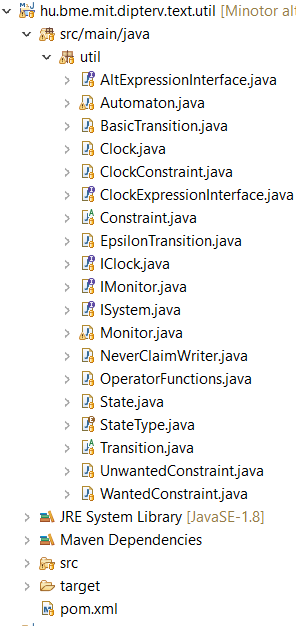
\includegraphics[width=180mm, height= 13cm, keepaspectratio]{figures/util_csomag.png}
    \caption{A \textit{util} csomag tartalma.}
	\label{util_csomag}
\end{figure}

A szükséges forráskódok generálásához az \textit{Xtend} technológiát használtam.

%----------------------------------------------------------------------------
\clearpage\subsection{Mintapélda}
%----------------------------------------------------------------------------

A \ref{mintapélda} kódrészleten látható egy szcenárió követelmény szöveges leírása, amit egy okostelefon működésére specifikáltunk.
A \ref{monitor_visualisation} ábrán látható a leíráshoz tartozó diagram vizualizációja, az \ref{okos_nc} kódrészlet pedig a generált automata leírását tartalmazza.

Az okostelefonon van egy zene lejátszási lista generáló alkalmazás.
A követelményben azt várjuk el, hogy ha a felhasználó megnyitja az alkalmazást akkor az előlapi kamera készít az arcáról egy képet.
A kép alapján eldönti, hogy milyen a felhasználó kedve és az alapján előállít egy zene lejátszási listát.

A \ref{okos_kapcsolat} kódrészleten látható az okostelefon és a monitor közti kapcsolat megvalósítása \textit{Java} kódban.
A rendszerben lévő \textit{User}, \textit{Device} és \textit{Database} osztályok mind attribútumként átveszik a \textit{Monitor} osztályt, amely megvalósítja az \textit{IMonitor} interfészt.

\begin{lstlisting}[frame=single, float=ht!, caption={Okostelefon működésére megadott szcenárió követelmény.},captionpos=b, label=mintapélda]
specification Photo{

	object User user;
	object Device device;
	object Database db;

	constraint error {
		message closeApp() user -> device;
	}

	scenario playlist_generation{
		message openApp() user -> device;
		message accessWebcam() device -> device;
		required message getPhoto() device -> user;
		fail message cameraOffline() user -> device;
		required strict message retrieveMood() device -> db;
		required message retrieveMusic() device -> db;
		strict message generatePlaylist() db -> device;
	}
}
\end{lstlisting}

\begin{figure}[!ht]
    \centering
    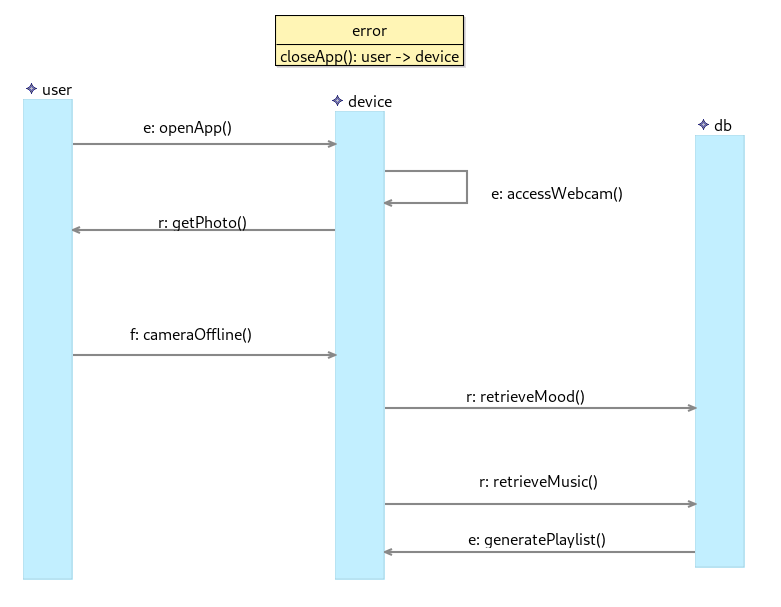
\includegraphics[width=150mm, keepaspectratio]{figures/monitor_device_visualisation_diagram.png}
    \caption{A \ref{mintapélda} leíráshoz tartozó diagram.}
	\label{monitor_visualisation}
\end{figure}

\begin{lstlisting}[frame=single, float=ht!, caption={Generált automata \textit{Never claim} formátumban.},captionpos=b,label=okos_nc]
never{ /*playlist_generationMonitor*/
T0_init:
 if
 :: (!(user.openApp().device)) -> goto T0_init
 :: (user.openApp().device) -> goto T0_q1
 fi;
T0_q1:
 if
 :: (!(device.accessWebcam().device)) -> goto T0_q1
 :: (device.accessWebcam().device) -> goto T0_q2
 fi;
T0_q2:
 if
 :: (!(device.getPhoto().user)) -> goto T0_q2
 :: (!(device.getPhoto().user)) -> goto accept_q3
 :: (device.getPhoto().user) -> goto T0_q4
 fi;
accept_q3:
 if
 fi;
T0_q4:
 if
 :: (!(user.cameraOffline().device)) -> goto T0_q6
 :: (!(user.cameraOffline().device)) -> goto T0_q4
 :: (user.cameraOffline().device) -> goto accept_q5
 fi;
accept_q5:
 if
 fi;
T0_q6:
 if
 :: (device.retrieveMood().db) -> goto T0_q8
 :: (!(device.retrieveMood().db)) -> goto accept_q7
 fi;
accept_q7:
 if
 fi;
T0_q8:
 if
 :: (!(device.retrieveMusic().db)) -> goto T0_q8
 :: (!(device.retrieveMusic().db)) -> goto accept_q9
 :: (device.retrieveMusic().db) -> goto T0_q10
 fi;
accept_q9:
 if
 fi;
T0_q10:
 if
 :: (db.generatePlaylist().device) -> goto T0_q11
 fi;
T0_q11:
 if
 fi;
}
\end{lstlisting}

\begin{lstlisting}[language=java, frame=single, float=ht!, caption={Az okostelefon és hozzá tartozó monitor fel konfigurálásának \textit{Java} implementációja.},captionpos=b,label=okos_kapcsolat]
public class Main {
	public static void monitorStatus(String status) {
		System.out.println(status);
	}

	public static void main(String[] args) {
		Specification specification = new Specification();
		specification.listAutomatas();
		IMonitor monitor = new Monitor(specification.getAutomata().get(0));

		User user = new User();
		Device device = new Device();
		Database db = new Database();
		user.device = device;
		device.user = user;
		device.db = db;
		db.device = device;
		user.monitor = monitor;
		device.monitor = monitor;
		db.monitor = monitor;

		user.init();
	}
}
\end{lstlisting}

\begin{lstlisting}[language=java, frame=single, float=ht!, caption={Az okostelefon \textit{Java} osztálya.},captionpos=b,label=okos_device]
public class Device {
	public IMonitor monitor;
	public User user;
	public Database db;

	void openApp() {
		monitor.update("user", "device", "openApp", new HashMap<String, Object>());
		accessWebcam();
	}

	void accessWebcam() {
		monitor.update("device", "device", "accessWebcam", new HashMap<String, Object>());
		user.getPhoto();
		db.retrieveMood();
		db.retrieveMusic();
	}

	void cameraOffline() {
		monitor.update("user", "device", "cameOffline", new HashMap<String, Object>());
	}

	void generatePlaylist() {
		monitor.update("db", "device", "generatePlaylist", new HashMap<String, Object>());
	}
}
\end{lstlisting}

A \ref{okos_device} kódrészlet az okostelefon \textit{Java} osztálya.
Megtekinthető a monitor és az eszköz közti kommunikáció megvalósítása is.
A \textit{Device} osztály a tágváltozójaként tárolt \textit{IMonitor}-nak küldi az üzeneteket az \textit{update()} függvény használatával.

\begin{lstlisting}[language=java, frame=single, float=ht!, caption={Monitor kimenete a rendszer működésének egyes fázisaiban.},captionpos=b,label=okos_monitor]
Received Message: user.openApp().device
q1
[System] Received status from monitor: System is in good state.
[Clock] reset x
Received Message: device.accessWebcam().device
q2
[System] Received status from monitor: System is in good state.
Received Message: device.getPhoto().user
q5
[System] Received status from monitor: System is in good state.
Received Message: someone.message().else
q7
[System] Received status from monitor: System is in good state.
Received Message: device.retrieveMood().db
q9
[System] Received status from monitor: System is in good state.
Received Message: device.retrieveMusic().db
q11
[System] Received status from monitor: System is in good state.
Received Message: db.generatePlaylist().device
q12
[System] Received status from monitor: System is in good state.
[System] Received status from monitor: Requirement satisfied
\end{lstlisting}

A \ref{okos_monitor} kódrészleten látszik, hogy a rendszer a működése elején nem felelt meg a monitor követelményének.
Amikor a működése végére ért, akkor a monitor jelezte, hogy a rendszer jó állapotban van a „\textit{Good state}” üzenettel és, hogy a követelmény teljesült a "\textit{Requirement Satisfied}" üzenettel.
A mintapéldához tartozó \textit{Specification} osztály a \textit{Függelékben} található (\ref{specification_class}), amelynek a konstruktorában található a generált időzített automata.

%----------------------------------------------------------------------------
\clearpage\subsection{Összetett szerkezetek}
%----------------------------------------------------------------------------

A monitor forráskód generátor támogatja az \textit{alt}, \textit{par} vagy \textit{loop} operátorokat tartalmazó szcenáriókat is.
Ezt a funkcionalitást a tesztelés során mutatom be részletesebben.

%----------------------------------------------------------------------------
\subsection{Időzítési feltételek}
%----------------------------------------------------------------------------

A monitor forráskód generátor támogatja az időzítési feltételeket tartalmazó szcenáriókat is.
A \ref{computer_scenario} kódrészletben található szcenárió első üzenetén a "\textit{reset x}" címke jelzi a monitornak, hogy az "\textit{x}" óraváltozót nullázni kell.
Egy óraváltozó felvételét is a "\textit{reset}" címkével lehet végrehajtani.
Ezt az óraváltozót használhatjuk majd a szcenáriónk későbbi üzeneteinél időzítési feltételek megadására.
Például a \ref{computer_scenario} kódrészletben levő szcenárió esetén, ha a monitor megkapja a \textit{checkEmail()} üzenetet, akkor létrehozz egy "\textit{x}" óraváltozót mivel ilyen még nem létezett előtte.
Ha a szcenárió végére érünk és a monitor megkapja a \textit{downloadEmail()} üzenetet, akkor a monitor kiértékeli az üzeneten lévő időzítési feltételt az óraváltozóban tárolt időérték alapján.
Ha az előbbi feltétel teljesült akkor tovább lépteti az időzített automatát.
A \ref{computer_main} kódrészlet a példához tartozó \textit{Main} \textit{Java} osztály leírását tartalmazza, a \ref{computer_java} kódrészlet pedig a rendszerhez tartozó \textit{Computer} \textit{Java} osztályt.
A \ref{computer_monitor} kódrészleten megtekinthető a monitor kimenete.
A kimenet végén levő "\textit{System is in good state.}" üzenet jelzi, hogy a rendszer jó állapotban van.

\begin{lstlisting}[language=java, frame=single, float=ht!, caption={Időzítési feltételeket tartalmazó szcenárió},captionpos=b,label=computer_scenario]
specification Email {

	object Computer computer;
	object Server server;

	clock x;

	constraint constraints{
		message logout() computer -> server;
	}

	constraint c {
		message login() server -> computer;
	}

	scenario sendEmail{
		message checkEmail() computer -> computer reset x;
		message sendUnsentEmail() required computer -> server;
		message newEmail() computer -> server pastConstraint {constraints};
		message downloadEmail() computer -> server clockConstraint {x < 10};
	}
}
\end{lstlisting}

\begin{lstlisting}[language=java, frame=single, float=ht!, caption={Időzítéses példához tartozó \textit{Main} osztály.},captionpos=b,label=computer_main]
public class Main {
	public static void monitorStatus(String status) {
		System.out.println(status);
	}

	public static void main(String[] args) {
		Specification specification = new Specification();
		specification.listAutomatas();
		IClock clock = new Clock();
		IMonitor monitor = new Monitor(specification.getAutomata().get(0), clock);

		Server server = new Server(monitor);
		Computer computer = new Computer(server, monitor);
	}
}
\end{lstlisting}

\begin{lstlisting}[language=java, frame=single, float=ht!, caption={\textit{Computer} \textit{Java} osztály.},captionpos=b,label=computer_java]
public class Computer {
	public Server server;
	public IMonitor monitor;

	Computer(Server server, IMonitor monitor) {
		this.server = server;
		this.monitor = monitor;
		monitor.update("computer", "computer", "checkEmail", new HashMap<String, Object>());
		checkEmail();
	}

	void checkEmail() {
		monitor.update("computer", "server", "sendUnsentEmail", new HashMap<String, Object>());
		server.sendUnsentEmail();

		monitor.update("computer", "server", "newEmail", new HashMap<String, Object>());
		server.newEmail();

		monitor.update("computer", "server", "downloadEmail", new HashMap<String, Object>());
		server.downloadEmail();
	}
}
\end{lstlisting}

\begin{lstlisting}[language=java, frame=single, float=ht!, caption={Időzítéses példa monitor kimenete.},captionpos=b,label=computer_monitor]
Received Message: computer.checkEmail().computer
q1
[System]Received status from monitor: System is in good state.
Received Message: computer.sendUnsentEmail().server
q3
[System]Received status from monitor: System is in good state.
Received Message: computer.newEmail(receiver, subject).server
q4
[System]Received status from monitor: System is in good state.
Received Message: computer.downloadEmail(timeout).server
q5
[System]Received status from monitor: System is in good state.
[System]Received status from monitor: Requirement satisfied
\end{lstlisting}

Az óraváltozók és időzítések megvalósításához az "\textit{org.apache.commons.lang3}" \cite{Maven} könyvtár "\textit{time}" csomag \textit{StopWatch} osztályát használtam.
Ha az automata élén van egy időzítési feltétel, akkor a monitor komponens az időzítő komponenstől elkéri a feltételben szereplő óraváltozóban tárolt időt és kiértekeli a feltételt.
Ha a feltétel teljesül, akkor az időzítés szempontjából a tranzíció megtörténhet.
A monitor akkor jelez hibát, ha az átmeneten lévő időzítési feltétel nem teljesült és az üzenet más átmenetre sem illeszkedik.
%----------------------------------------------------------------------------
\chapter{Tesztelési terv}
%----------------------------------------------------------------------------

%----------------------------------------------------------------------------
\section{Tesztelési célok}
%----------------------------------------------------------------------------

A generált monitor forráskód tesztelésére a következő célokat fogalmazuk meg:

\begin{itemize}
    \item Az összes üzenet típus megjelenése a különböző teszt szenáriókban
    \item Időzített feltételek helyes kiértékelése
    \item Üzenet megkötések tesztelése
    \item Alt és Par operátorok esetén, az üzenet szekvencia ágak helyes kiértékelése
    \item Loop operátor esetén a minimális és maximálás üzenet ismétlődések tesztelése
    \item Összetett szenárió tesztelése, ami több operátort tartalmaz
    \item Egymást követő elvárt üzeneteket tartalmazó szenárió tesztelése
    \item Egymást követő fail üzeneteket tartalmazó szenárió tesztelése
    \item Regular üzenet tesztelése (ha megjelenik a rendszer működésében akkor ki kell értékelni a szenárió többi részét, ha nem jelenik meg a monitor helyes működést kell jelezzen és, hogy a követelmény nem teljesült)
    \item Több óraváltozót tartalmazó szenárió tesztelése
    \item Egymást követő üzenetek kombinációinak tesztelése (pl. elvárt üzenetet követő fail, elvárt üzenetet követő reguláris, stb.)
\end{itemize}

%----------------------------------------------------------------------------
\clearpage\section{Monitor forráskód generátor tesztelése}
%----------------------------------------------------------------------------

A generált monitor forráskodját integrációs tesztek segítségével szeretnénk tesztelni.
A teszteinkben egy példa rendszer java implementációját integráljuk a generált monitor komponenssel.
Az Xtext keretrendszer a specifikált DSL (Domain Specific Language) nyelvhez generál egy Maven plugin-t.
Ezt a plugin-t betölthetjük egy egyszerű maven projektbe és használhatjuk is az elkészített DSL nyelvünket, azaz létrehozhatunk a projektben a saját DSL-ünkhöz tartozó fájlokat, melyekben megadhatjuk saját scenario-inkat.

\begin{figure}[!ht]
    \centering
    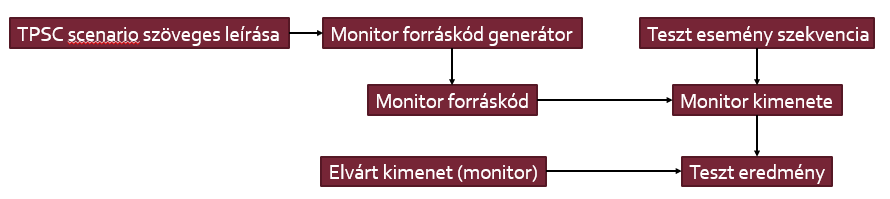
\includegraphics[width=150mm, height=9cm, keepaspectratio]{figures/integration_test_flow.png}
    \caption{Integrációs tesztelés folyamatábrája.}
\end{figure}

A 9.2. ábrán megtekinthető az integrációs tesztelés tervének folyamatábrája.
A következők tesztelési kategoriáink:

\begin{itemize}
    \item Scenario operátorok tesztelése
    \item Üzenet paraméterek tesztelése
    \item Időzítések tesztelése
\end{itemize}

A scenario operátorok tesztelésénél az a célunk, hogy a monitor a követelmény különböző ágait figyelembe véve helyes kimenetet adjon.
Például loop operátor esetén a minimum, köztes és maximum üzenet szekvencia ismétléseknél is helyes legyen a monitor kimenete.
Ha a maximumnál többször szerepel az üzenet szekvencia akkor hibát kell, hogy jelezen.
Üzenet paraméterek tesztelése esetén azt szeretnénk vizsgálni, hogy a monitor helyesen értelmezi e az üzenet paramétereket.
Az időzítések tesztelésénél az a fontos, hogy a monitor képes-e az óraváltozók alapján az időzitési feltételeket kiértékelni.
Például ha az üzenet a feltétel alapján időben érkezik meg akkor helyes kimenetet adjon vissza ha feltétel szerint később érkezik meg akkor a monitornak hibát kell jeleznie.

Egy integrációs teszt akkor sikeres ha a monitor kimenete megegyezik az elvárt kimenettel.
Az elvárt kimenetet a rendszer manuális tesztelése határoz meg.
A tesztelő dönti el, hogy helyesen kell hogy működjön vagy sem amit a monitornak jeleznie kell.

%----------------------------------------------------------------------------
\clearpage
%----------------------------------------------------------------------------

Az Xtext keretrendszer a definiált DSL nyelvünkhöz generál egy Maven projekt architektúrát.
A nyelvünk így elérhető maven plugin formájában is, amit felhasználhatunk az integrációs teszteinkhez.
Elég csupán egy maven projektet felkonfigurálni a saját dsl plugin-ünkkel és elkészítethetjük a saját tesztelési keretrendszerünket.
Ezek a maven projektek a szülő projektünkben helyezkedhetnek el, így a projekt struktúrában közvetlen a nyelvünk mellett vannak.
A 9.3. ábrán és a 9.1. kódrészléten látható egy ilyen integrációs teszthez tartozó maven projekt felépítése és a hozzá tartozó teszteset.

\begin{figure}[!ht]
    \centering
    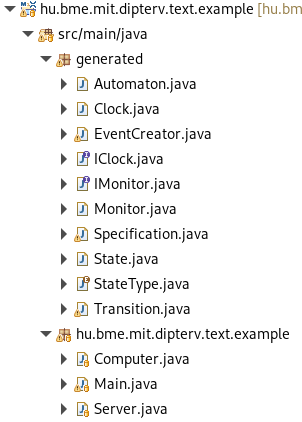
\includegraphics[width=150mm, height=9cm, keepaspectratio]{figures/integration_test_structure.png}
    \caption{Példa integrációs teszt projekt struktúrája.}
\end{figure}

A 9.3. ábrán lévő \textit{generated} csomag tartalmazza a scenariohoz tartozó generált automata forráskódját és a monitor forráskódját.
A \textit{hu.bme.mit.dipterv.text.example} csomag a tesztelt rendszer \textit{Java} implementációját tartalmazza.

\begin{lstlisting}[language=java, frame=single, float=ht!, caption={Integrációs teszteset.},captionpos=b]
package hu.bme.mit.dipterv.text.example;

import org.junit.jupiter.api.Test;
import org.junit.jupiter.api.Assertions;

import generated.Specification;
import generated.IClock;
import generated.IMonitor;
import generated.Monitor;
import generated.Clock;

public class MonitorPassingTest {

	@Test
	public void testMonitorPassing() {
		Specification specification = new Specification();
		specification.listAutomatas();
		IClock clock = new Clock();
		IMonitor monitor = new Monitor(specification.getAutomata().get(0), clock);

		Server server = new Server(monitor);
		Computer computer = new Computer(server, monitor);
		Assertions.assertTrue(monitor.goodStateReached());
	}
}
\end{lstlisting}

\begin{lstlisting}[language=java, frame=single, float=ht!, caption={Integrációs teszteset eredménye.},captionpos=b]
-------------------------------------------------------
T E S T S
-------------------------------------------------------
Running hu.bme.mit.dipterv.text.example.MonitorPassingTest
q0 NORMAL
q1 NORMAL
q2 ACCEPT
q3 NORMAL
q4 NORMAL
q5 FINAL
!(computer.checkEmail().computer) q0->q0
computer.checkEmail().computer q0->q1
!(computer.sendUnsentEmail().server) q1->q1
!(computer.sendUnsentEmail().server) q1->q2
computer.sendUnsentEmail().server q1->q3
!(computer.logout().server) & !(computer.newEmail().server) q3->q3
computer.newEmail().server q3->q4
!(computer.downloadEmail().server) q4->q4
computer.downloadEmail().server q4->q5
Received Message: computer.checkEmail().computer
Transition: !(computer.checkEmail().computer)
Transition: computer.checkEmail().computer
transition triggered: computer.checkEmail().computer
q1

Received Message: computer.sendUnsentEmail().server
Transition: !(computer.sendUnsentEmail().server)
Transition: !(computer.sendUnsentEmail().server)
Transition: computer.sendUnsentEmail().server
transition triggered: computer.sendUnsentEmail().server
q3

Received Message: computer.newEmail().server
Transition: !(computer.logout().server) & !(computer.newEmail().server)
Transition: computer.newEmail().server
transition triggered: computer.newEmail().server
q4

Received Message: computer.downloadEmail().server
Transition: !(computer.downloadEmail().server)
Transition: computer.downloadEmail().server
transition triggered: computer.downloadEmail().server
q5

Tests run: 1, Failures: 0, Errors: 0, Skipped: 0, Time elapsed: 0.025 sec

Results :

Tests run: 1, Failures: 0, Errors: 0, Skipped: 0
\end{lstlisting}

A 9.2. kódrészlet a Maven teszt kimenetét tartalmazza.

Ezt a projekt struktúrát felhasználva a teszteink köré tudunk egy Maven alapú Continuous Integration-t (CI) állítani.

A függelékben található egy példa unit teszt eset az automata generátor tesztelésére.

%----------------------------------------------------------------------------
\clearpage\section{Continuous Integration}\subsection{Github Actions CI}
%----------------------------------------------------------------------------

Az időzített automata és monitor forráskód generátorok automatikus tesztelése a Github Actions segítségével történik.
A CI minden feltöltött új commit esetén lefut.
A CI különböző fázisai a következők:

\begin{itemize}
    \item I. Teljes Xtext projekt fordítása (Maven)
    \item II. Intergrációs tesztek futtatása
\end{itemize}

A generátorokhoz tartozó Xtext projekten lefut egy Maven build, amely az új feltöltött verzió tartalmazza.
Ez a build állítja elő a DSL nyelvhez tartozó Maven plugin-t is.
A fordítással együtt lefutnak a unit tesztek is.
Ezt követően hajtódnak végre az integrációs tesztek, amelyek a frissen fordított Maven plugint használják.
Ha az összes fázis sikeresen lefutott, akkor az adott commit nem rontott el semmilyen korábbi funkciót.
A CI-hoz tartozó script-et a 9.3. kódrészlet tartalmazza.

\begin{figure}[!ht]
    \centering
    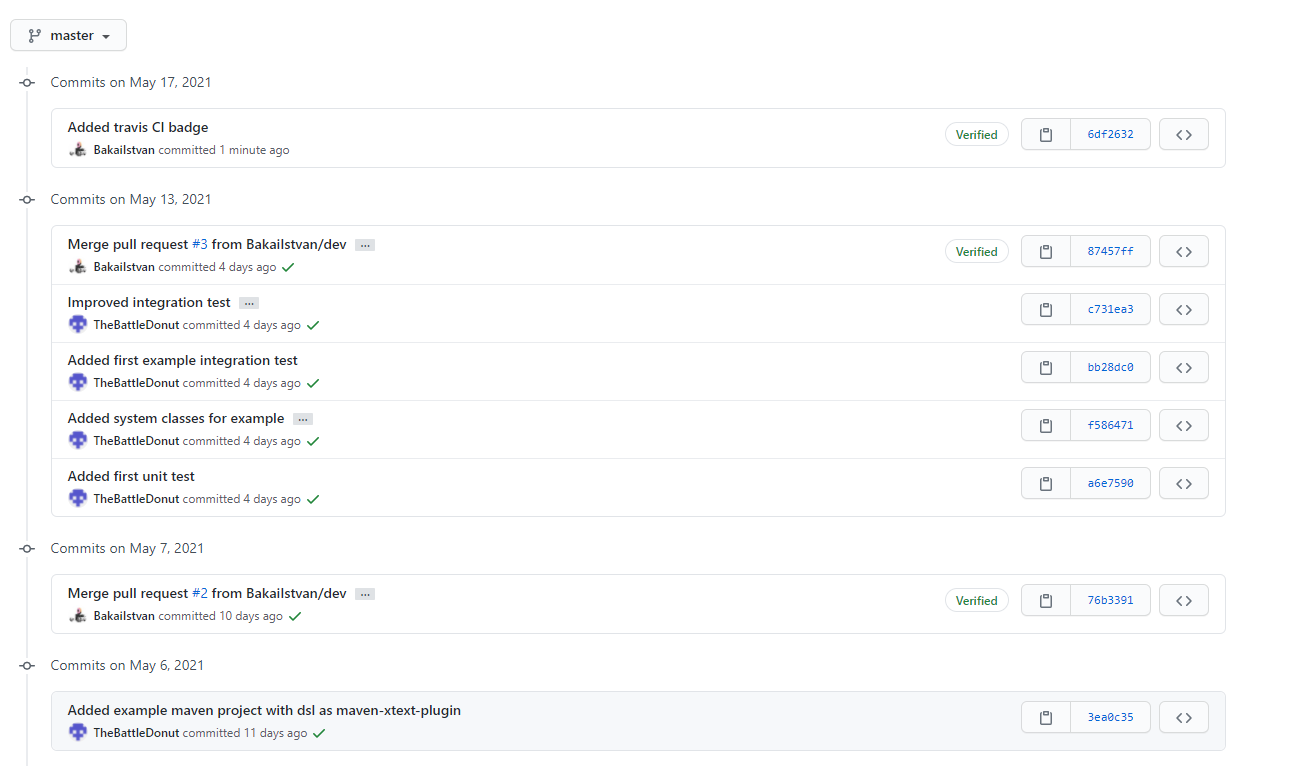
\includegraphics[width=150mm, keepaspectratio]{figures/github_ci_check.png}
    \caption{GitHub repository commit-ok és hozzá tartozó CI check-ek.}
\end{figure}

\begin{figure}[!ht]
    \centering
    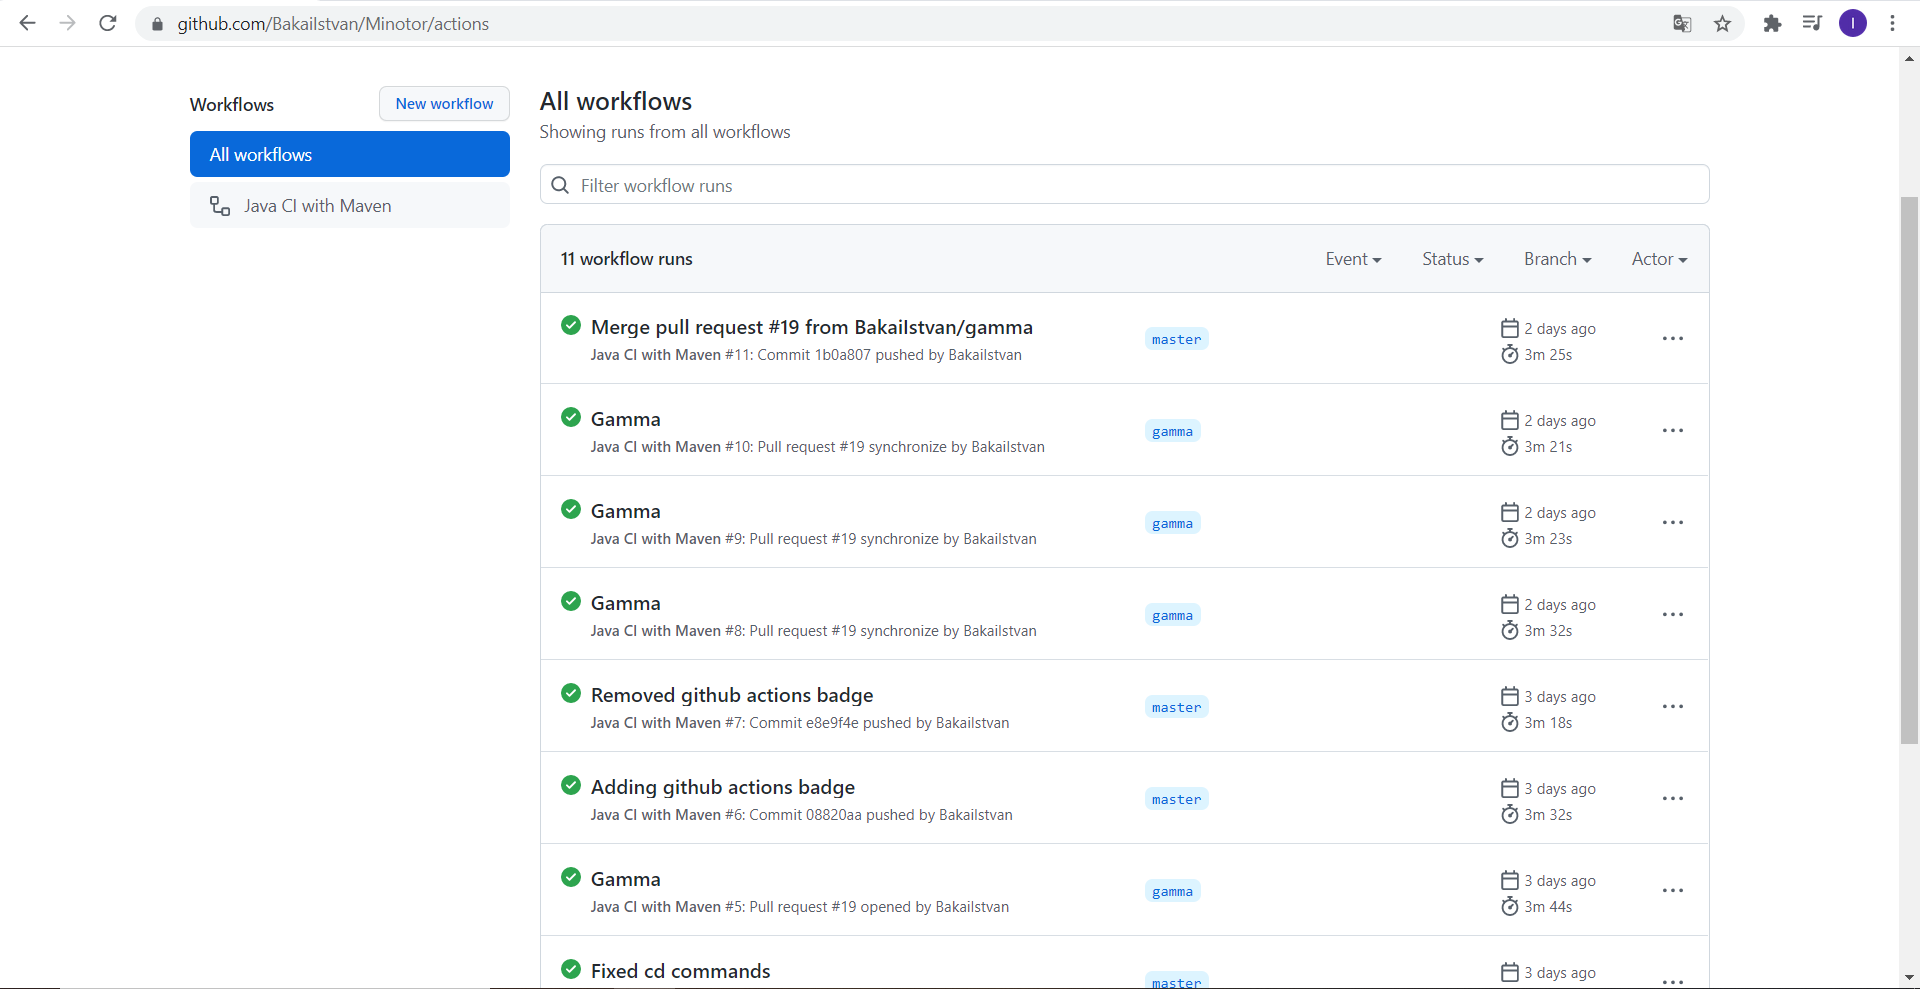
\includegraphics[width=150mm, keepaspectratio]{figures/github_ci_builds.png}
    \caption{Github Actions CI build-ek eredményei.}
\end{figure}

\begin{lstlisting}[language=java, frame=single, float=ht!, caption={Github Actions CI-hoz tartozó .yml script.},captionpos=b]
# This workflow will build a Java project with Maven, and cache/restore any dependencies to improve the workflow execution time
# For more information see: https://help.github.com/actions/language-and-framework-guides/building-and-testing-java-with-maven

name: Java CI with Maven

on:
    push:
    branches: [ master ]
    pull_request:
    branches: [ master ]

jobs:
    build:

    runs-on: ubuntu-latest

    steps:
    - uses: actions/checkout@v2
    - name: Set up JDK 11
        uses: actions/setup-java@v2
        with:
        java-version: '11'
        distribution: 'adopt'
        cache: maven
    - name: Build with Maven
        run: mvn clean install -U
    - name: Test example project
        run: cd hu.bme.mit.dipterv.text.example; mvn clean install -U
    - name: Test mobileexample project
        run: cd hu.bme.mit.dipterv.text.mobileexample; mvn clean install -U
    - name: Test altexample project
        run: cd hu.bme.mit.dipterv.text.altexample; mvn clean install -U
    - name: Test parexample project
        run: cd hu.bme.mit.dipterv.text.parexample; mvn clean install -U
    - name: Test operatorexample project
        run: cd hu.bme.mit.dipterv.text.operatorexample; mvn clean install -U
    - name: Test gamma integration project
        run: cd hu.bme.mit.dipterv.text.gammaexample; mvn clean install -U
\end{lstlisting}

%----------------------------------------------------------------------------
\clearpage\section{Tesztesetek}\subsection{Egyszerű időzítési megkötéseket tartalmazó tesztszenárió}
%----------------------------------------------------------------------------

A tesztesetekhez tartozó scenario követelmény megtalálható az x. ábrán.

\begin{lstlisting}[language=java, frame=single, float=ht!, caption={Integrációs teszteset.},captionpos=b]
specification Email {

	object Computer computer;
	object Server server;

	integer timeout = 10;
	string receiver = "John";
	string subject = "Next meeting";

	clock x;

	constraint constraints {
		message logout() computer -> server;
	}

	scenario sendEmail{
		message checkEmail() computer -> computer reset x;
		required message sendUnsentEmail() computer -> server;
		pastConstraint {constraints} message newEmail(receiver, subject) computer -> server;
		message downloadEmail(timeout) computer -> server clockConstraint {>(x,10)};
	}
}
\end{lstlisting}

\begin{figure}[!ht]
    \centering
    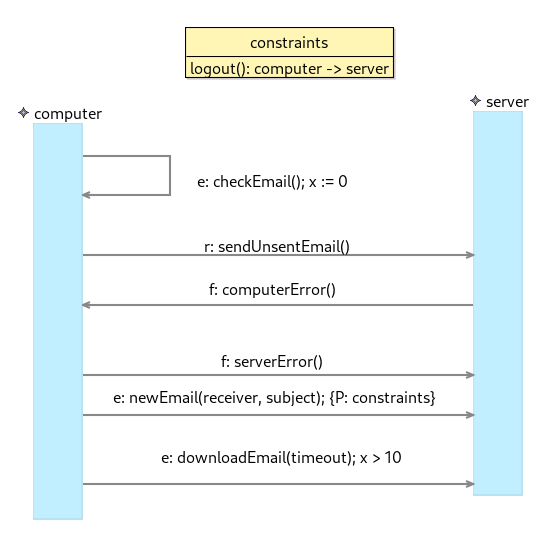
\includegraphics[width=150mm, keepaspectratio]{figures/diagramExample.png}
    \caption{Szenárió diagram.}
\end{figure}

A rendszerben egy szervergépből és egy felhasználói számitogépből áll.
A szerver egy e-mail szervert szimulál, aminek a számitogép különböző kéréseket küldhet.
Például lekérdezheti tőle a kapott e-mail vagy új e-mail küldhet.
A követelményben leírjuk, hogy a rendszernek mi a helyes viselkedése e-mail küldés esetén.
Ha a computer a \textit{checkEmail} hívást használva talál elküldendő e-mail az továbbítja a szervernek.
Ezt az \textit{elvárt} \textit{sendUnsentEmail} üzenet jelzi.
Ezt követően meg kell jelenjen a rendszer működésében a \textit{newEmail} üzenet.
A ehelyett \textit{logout} üzenet érkezik a hibás működést jelent.
A \textit{newEmail} üzenetet a \textit{downloadEmail} üzenet követi.
Ezen az üzeneten van egy 10 másodperces időzítési feltétel, ami a letöltést szimulálja.

A szenárióhoz tartozó tesztesetek a következők:

\begin{itemize}
    \item testNetworkRequirementSatisfied
    \item testNetworkNoErrors
    \item testNetworkWithErrors
    \item testNetworkWithNoDelay
    \item testNetworkFirstFail
    \item testNetworkSecondFail
\end{itemize}

A \textit{testNetworkRequirementSatisfied} tesztesetben a rendszer helyes működését szimuláljuk és azt ellenőrizzük, hogy a generált monitor képes ezt érzékelni és jelzi.
A \textit{testNetworkNoErrors} azt vizsgálja, hogy a monitor képes-e érzékelni, hogy a rendszer nem felelt meg a követelménynek.
Itt úgy manipuláljuk a teszt rendszer, hogy lehagyjuk a letöltés részt a működésből.
Ilyenkor a rendszer nem felel meg a követelménynek, viszont még jó állapotban marad, mert nem történt hiba.
A \textit{testNetworkWithErrors} tesztesetnél a \textit{sendUnsentEmail} üzenet után egy \textit{logout} üzenetet küldünk a monitor és azt vizsgáljuk képes-e detektálni ezt a hibát.
A \textit{testNetworkWithNoDelay}-nél pedig túl gyorsan küldjük a működés végén a \textit{downloadEmail} üzenetet és azt ellenőrizzük képes e a monitor ezt a hibát érzékelni.

%----------------------------------------------------------------------------
\clearpage\subsection{Többféle üzenetet és megkötést tartalmazó egyszerű tesztszenárió}
%----------------------------------------------------------------------------

\begin{lstlisting}[language=java, frame=single, float=ht!, caption={Integrációs teszteset.},captionpos=b]
    specification Photo{

        object User user;
        object Device device;
        object Database db;

        clock x;

        constraint error {
            message closeApp() user -> device;
        }

        scenario playlist_generation{
            message openApp() user -> device reset x;
            message accessWebcam() device -> device clockConstraint {<=(x, 5)} reset x;
            required futureConstraint {error} message getPhoto() device -> user;
            fail message cameraOffline() user -> device;
            required strict message retrieveMood() device -> db;
            required message retrieveMusic() device -> db;
            strict message generatePlaylist() db -> device clockConstraint {<(x, 15)};
        }
    }
\end{lstlisting}

\begin{figure}[!ht]
    \centering
    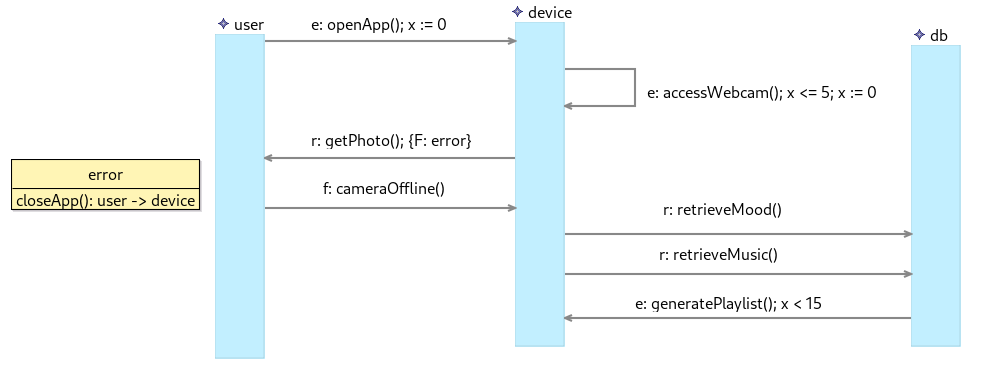
\includegraphics[width=150mm, keepaspectratio]{figures/diagramMobileExample.png}
    \caption{Szenárió diagram.}
\end{figure}

A tesztrendszerünk egy zene lista generáló alkalmazás, ami egy felhasználót, mobileszközt és adatbázist tartalmaz.
A felhasználó "kedve" alapján generálja a listát, amit az arc kifejezése alapján határoz meg.
A követelményben a rendszer alap működése van leírva egészen az elejétől, amikor a felhasználó megnyítja az alkalmazást.
A követelmény leírás megtekinthető az x. ábrán.

A szenárióhoz tartozó tesztesetek a következők:

\begin{itemize}
    \item testMobileRequirementSatisfied
    \item testMobileFutureConstraint
    \item testMobileFutureConstraintEarly
    \item testMobileWithError
    \item testMobileWithDelay
    \item testMobileWithTooMuchDelay
    \item testMobileMissingRequiredMessage
    \item testMobileRequiredEventually
    \item testMobileRequiredNotReceived
\end{itemize}

A teszteseteket a monitor hiba detektáló képeségét tesztelik.
A \textit{testMobileWithDelay} és \textit{testMobileWithTooMuchDelay} tesztesetek az \textit{x <= 5} időzítési feltétel beteljesülését ellenőrzik.
A \textit{testMobileWithDelay} 5 másodperces késleltetéssel küldjük az \textit{accessWebcam} üzenetet, míg a másiknál 6 másodperces késleltetéssel.
Az első esetben a monitornak helyes működést kell érzékelnie a következőben pedig hibás működést.

%----------------------------------------------------------------------------
\clearpage\subsection{Alt operátort tartalmazó tesztszenárió}
%----------------------------------------------------------------------------

A tesztszenárióhoz tartozó rendszerünk egy banki rendszer.
A szenárió megtalálható az x. ábrán.

\begin{lstlisting}[language=java, frame=single, float=ht!, caption={Integrációs teszteset.},captionpos=b]
specification Bank {

    object UserInterface ui;
    object ATM atm;
    object BankDB db;

    bool success = true;

    constraint b {
        message logout() ui->atm;
    }

    scenario transaction {
        message login(success) ui->atm;

        alt (equals(success, true)) {
            pastConstraint {b} message wReq() ui->atm;
            message uDB() atm->db;
        } (equals(success, false)) {
            message loginUnsuccessful() ui->atm;
            required message lockMachine() atm->ui;
        }
    }
}
\end{lstlisting}

\begin{figure}[!ht]
    \centering
    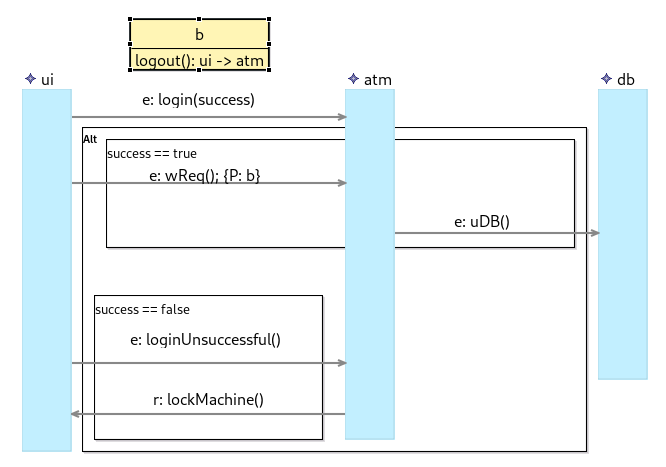
\includegraphics[width=150mm, keepaspectratio]{figures/diagramAltExample.png}
    \caption{Szenárió diagram.}
\end{figure}

A rendszer egy felhasználói felületből, ATM-ből és banki adatbázisból áll.
A követelményünkben két lehetséges működést írunk le.
A \textit{success} paraméter jelzi, hogy melyik működés a helyes.
A szenárióhoz tartozó tesztesetek a következők:

\begin{itemize}
    \item testBankMonitorPassing
    \item testBankMonitorFailing
    \item testBankMonitorFalseCasePassing
    \item testBankMonitorFalseCaseFailing
\end{itemize}

A tesztesetekkel azt vizsgáljuk, hogy a monitor képes-e a helytelen ág lefutását hibának érzékelni és a helyes viselkedés esetén detektálni a követelmény teljesítését.

%----------------------------------------------------------------------------
\clearpage\subsection{Par operátort tartalmazó tesztszenárió}
%----------------------------------------------------------------------------

\begin{lstlisting}[language=java, frame=single, float=ht!, caption={Integrációs teszteset.},captionpos=b]
specification Email {
    object Computer computer;
    object Server server;

    constraint constraints{
        message logout() computer -> server;
    }

    scenario email {
        par {
            case checkEmail {
                message checkEmail() computer -> computer;
            }

            case newEmail {
                pastConstraint {constraints} message newEmail() computer -> server;
            }
        }
    }
}
\end{lstlisting}

\begin{figure}[!ht]
    \centering
    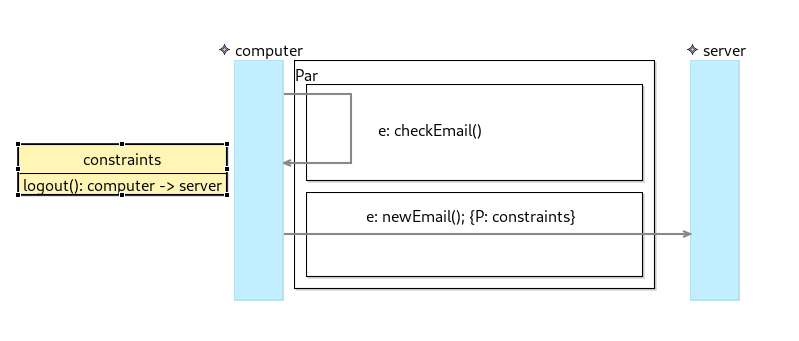
\includegraphics[width=150mm, keepaspectratio]{figures/diagramParExample.png}
    \caption{Szenárió diagram.}
\end{figure}

Ehhez a tesztszenárióhoz az első szenárióban lévő teszt rendszert használtuk fel.
A szenárióhoz tartozó tesztesetek a következők:

\begin{itemize}
    \item testNetworkRequirementSatisfied
    \item testNetworkOtherRequirementSatisfied
\end{itemize}

Azt vizsgáljuk, hogy a monitor képes mindkét permutáció esetén érzékelni a követelmény teljesítését.

%----------------------------------------------------------------------------
\clearpage\subsection{Komplex tesztszenárió loop és alt operátorokkal}
%----------------------------------------------------------------------------

\begin{lstlisting}[language=java, frame=single, float=ht!, caption={Integrációs teszteset.},captionpos=b]
specification Connection {

    object Computer computer;
    object Server server;

    string receiver = "John";
    string subject = "Next Meeting";
    bool success = false;

    clock x;
    clock y;

    constraint logout {
        message logout() computer -> server;
    }

    constraint delete {
        message deleteEmail(subject) computer -> server;
    }

    scenario authentication {
        loop (1, 3) {
            message login() computer -> computer reset x;
            pastConstraint {logout} message attemptLogin() computer -> server reset y;
        }

        alt (equals(success, true)) {
            message checkEmail() computer -> server clockConstraint {<(x, 2)};
            required futureConstraint {delete} message newEmail(receiver, subject) computer -> server reset x;
        } (equals(success, false)) {
            required message logoutUser() server -> computer clockConstraint {>(y, 3)};
            message lockComputer() server -> computer reset y;
        }
    }
}
\end{lstlisting}

\begin{figure}[!ht]
    \centering
    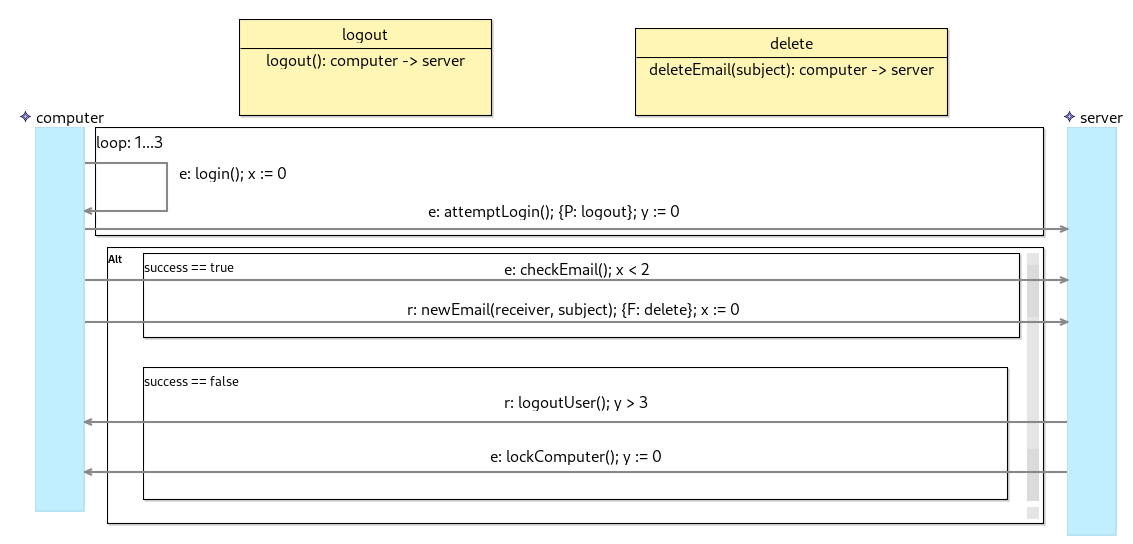
\includegraphics[width=150mm, keepaspectratio]{figures/diagramOperatorExample.png}
    \caption{Szenárió diagram.}
\end{figure}

\begin{itemize}
    \item testNetworkRequirementSatisfied
    \item testNetworkRequirementSatisfiedTwice
    \item testNetworkRequirementSatisfiedThreeTimes
    \item testNetworkRequirementSatisfiedFourTimes
    \item testNetworkAltTrueCase
    \item testNetworkAltTrueCaseSatisfied
    \item testNetworkLogoutTooFast
    \item testNetworkLogoutConstrait
\end{itemize}

\clearpage\section{Tesztelés összefoglaló}

\begin{longtable}{|p{0.1428\linewidth}|p{0.1428\linewidth}|p{0.1428\linewidth}|p{0.1428\linewidth}|p{0.1428\linewidth}|p{0.1428\linewidth}|}
\hline
\textbf{Tesztelési célok} & \textbf{Egyszerű tesztszenárió} & \textbf{Több üzenetet tartalmazó tesztszenárió} & \textbf{Alt operátort tartalmazó tesztszenárió} & \textbf{Par operátort tartalmazó tesztszenárió} & \textbf{Komplex tesztszenárió}\\
\hline
Egyszerű üzenet megjelenése & X & X & X & X & X\\
\hline
Elvárt üzenet megjelenése & X & X & X & - & X\\
\hline
Nem kivánt (fail) üzenet megjelenése & X & X & - & - & -\\
\hline
Strict üzenet tesztelése & - & X & - & - & -\\
\hline
Időzítési feltételek tesztelése & X & X & - & - & X\\
\hline
Past megkötés tesztelése & X & - & X & X & X\\
\hline
Future megkötés tesztelése & - & X & - & - & X\\
\hline
Alt operátor tesztelése & - & - & X & - & X\\
\hline
Par operátor tesztelése & - & - & - & X & -\\
\hline
Loop operátor tesztelése & - & - & - & - & X\\
\hline
Több operátort tartalmazó szenárió tesztelése & - & - & - & - & X\\
\hline
Egymást követő elvárt üzenetek & - & X & - & - & -\\
\hline
Egymást követő fail üzenetek & X & - & - & - & -\\
\hline
Sima üzenet tesztelése & X & X & X & X & X\\
\hline
Több óraváltozó & - & - & - & - & X\\
\hline
Elvárt után fail üzenet & X & - & - & - & -\\
\hline
Fail után elvárt üzenet & - & X & - & - & -\\
\hline
\caption{Összefoglaló táblázat}
\label{tab:table1}
\end{longtable}
%----------------------------------------------------------------------------
\chapter{TPSC specifikációk vizualizációja}
%----------------------------------------------------------------------------

A specifikációk vizualizációjához a \textit{Modell alapú rendszertervezés} tárgy során készített PSC vizualizációs Sirius alkalmazást használtam fel.
Előszőr kiegészítettem az alkalmazást TPSC elemek vizualizációjával.
Egy \textit{XML} generátor előállítja a specifikáció \textit{XMLs} leírását, amit a Sirius alkalmazás képes feldolgozni és előállítani a hozzá tartozó diagramot.

\begin{figure}[!ht]
    \centering
    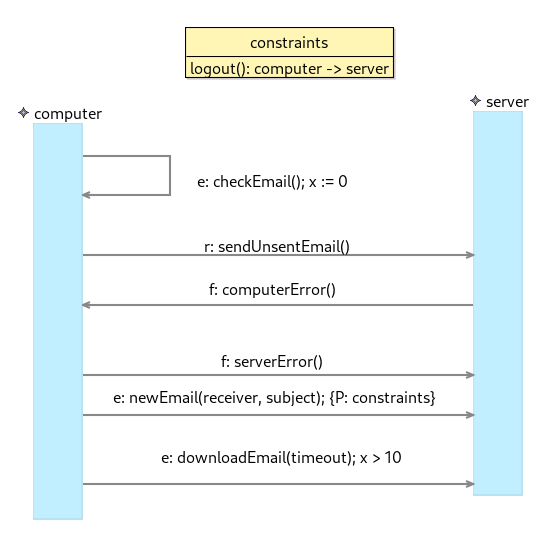
\includegraphics[width=150mm, keepaspectratio]{figures/diagramExample.png}
    \caption{Szenárió diagram.}
\end{figure}

\begin{lstlisting}[language=java, frame=single, float=ht!, caption={Szenárió diagram xml leírása.},captionpos=b]
<?xml version="1.0" encoding="UTF-8"?>
<minotor:SequenceDiagram xmi:version="2.0" xmlns:xmi="http://www.omg.org/XMI" xmlns:minotor="hu.bme.mit.mdsd.xboyz.erdiagram" Name="Email">

<lifelines Name="computer" Type="Computer"/>
<lifelines Name="server" Type="Server"/>

<constraints Name="constraints">
<transitions Name="logout()" source="//@lifelines.0" target="//@lifelines.1"/>
</constraints>

<transitions Name="checkEmail()" Type="REGULAR" Label="e: checkEmail()" source="//@lifelines.0" target="//@lifelines.0"  after="//@transitions.1" reset="x"/>
<transitions Name="sendUnsentEmail()" Type="REQUIRED" Label="r: sendUnsentEmail()" source="//@lifelines.0" target="//@lifelines.1" before="//@transitions.0" after="//@transitions.2"/>
<transitions Name="computerError()" Type="FAIL" Label="f: computerError()" source="//@lifelines.1" target="//@lifelines.0" before="//@transitions.1" after="//@transitions.3"/>
<transitions Name="serverError()" Type="FAIL" Label="f: serverError()" source="//@lifelines.0" target="//@lifelines.1" before="//@transitions.2" after="//@transitions.4"/>
<transitions Name="newEmail(receiver, subject)" Type="REGULAR" Label="e: newEmail(receiver, subject)" source="//@lifelines.0" target="//@lifelines.1" before="//@transitions.3" after="//@transitions.5" constraint="//@constraints.0" constraintType="PAST"/>
<transitions Name="downloadEmail(timeout)" Type="REGULAR" Label="e: downloadEmail(timeout)" source="//@lifelines.0" target="//@lifelines.1" before="//@transitions.4"   clockConstraint="x &gt; 10"/>
</minotor:SequenceDiagram>
\end{lstlisting}

A diagramon az egyes objektumok kék \textit{lifeline} formájában jelenek meg.
Minden üzenethez tartozik egy nyíl.
A nyíl címkéjére írjuk az üzenet összes tulajdonságát.
A nyíl eleje és vége \textit{lifeline}-okat kötnek össze, amik az üzenet feladóját és fogadóját jelzik.
A megkötéseket egy sárga táblázat formájában reprezentáljuk, amelybe bele írjuk az összes megkötésben szereplő üzenetet.

\begin{figure}[!ht]
    \centering
    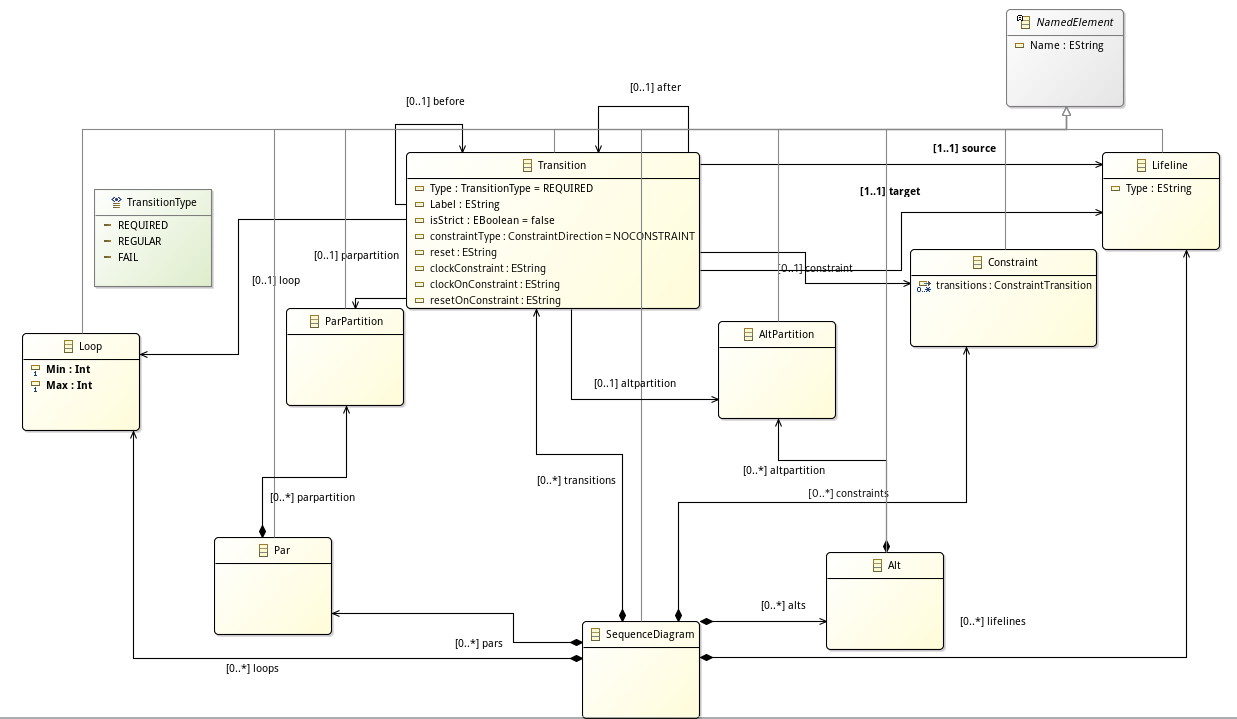
\includegraphics[width=150mm, keepaspectratio]{figures/sirius-minotor-erdiagram.png}
    \caption{Sirius alkalmazáshoz tartozó model ER diagramja.}
\end{figure}

\begin{figure}[!ht]
    \centering
    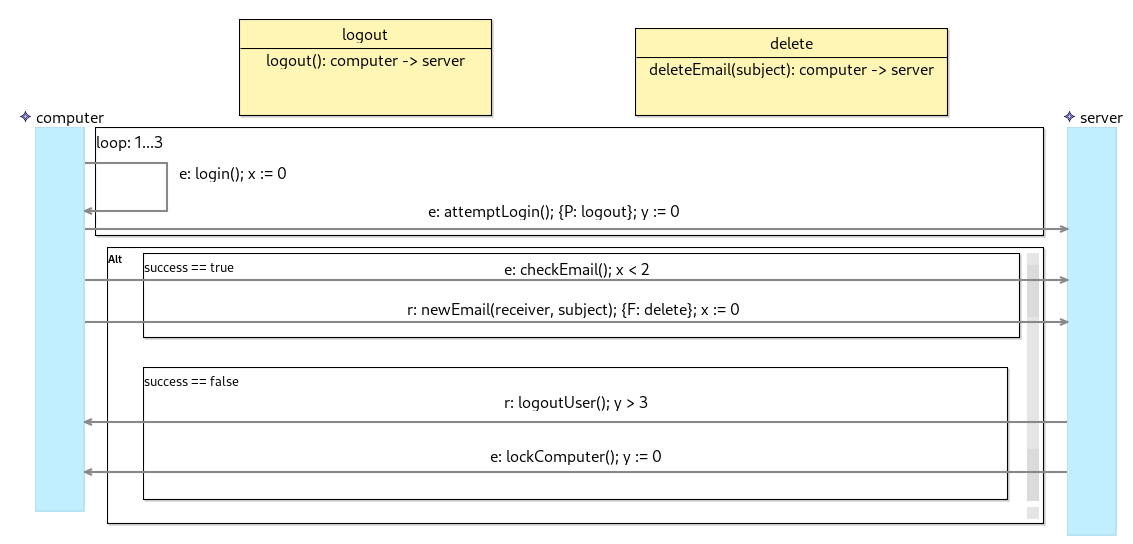
\includegraphics[width=150mm, keepaspectratio]{figures/diagramOperatorExample.png}
    \caption{Operátorokat tartalmazó szenárió diagram.}
\end{figure}

A diagramon keretek formájában jelenek meg az operátorok.
%----------------------------------------------------------------------------
\chapter{A monitor integrálása a Gamma keretrendszerben tervezett komponensekkel}
%----------------------------------------------------------------------------

\section{Gamma keretrendszer}

A \textit{Gamma} keretrendszerrel komponensalapú reaktív rendszereket lehet tervezni, és az a célja hogy támogassa az elosztott rendszerek modelallapú fejlesztését.
A létrehozott rendszert a keretrendszerrel lehet tesztelni, ellenőrizni és szimulálni is.
A keretrendszernek a \textit{Yakindu} modellező eszköz használja, amit kiegészít egy modellező réteggel ahol meg valósítható a komponensek közti kommunikációs hálózat.
A komponensek hierarchikusan helyezkednek el egymás mellett, ami megkönnyíti egyes komponensek többszöri felhasználását.
A tervezett rendszerhez a keretrendszer képes \textit{Java} forráskódot is generálni.
A modelhez generálhatoak tesztesetek vagy akár verifikálható az \textit{UPPAAL} model ellenőrző eszköz használatával.

A monitor illesztéséhez a \textit{Gamma} \textit{tutorial} csomagjában lévő rendszert használtam.
Ez egy irányitórendszer modelje, ami egy kereszteződésben lévő közlekedési lámpák működtetésért felel.
A jelző lámpák általános három fokozatú lámpák és a piros-zöld-sárga-piros jelzéseket ismétlik.
A rendszer támogat még egy megszakító állapotot, amit a rendőrség kapcsolhat be.
Ilyenkor minden lámpa sárgán villog.

\clearpage\section{Generált monitor integrációja}

A keretrendszer a \textit{gamma.monitor} csomagba generálja a beépített monitor forráskódja.
Ezt a \textit{Gamma} monitort cseréltem le a saját a monitor komponensemhez tartozó forráskóddal megvalósítva a szükséges interfészeket.

\begin{lstlisting}[language=java, frame=single, float=ht!, caption={Monitor komponenshez tartozó kódrészlet.},captionpos=b]
public void runComponent() {
    Queue<Event> eventQueue = getProcessQueue();
    while (!eventQueue.isEmpty()) {
            Event event = eventQueue.remove();
            switch (event.getEvent()) {
                case "LightInputs.DisplayNone":
                    update("controller", "light", "displayNone", new HashMap<String, Object>());
                break;
                case "LightInputs.DisplayYellow":
                    update("controller", "light", "displayYellow", new HashMap<String, Object>());
                break;
                case "LightInputs.DisplayRed":
                    update("controller", "light", "displayRed", new HashMap<String, Object>());
                break;
                case "LightInputs.DisplayGreen":
                    update("controller", "light", "displayGreen", new HashMap<String, Object>());
                break;
                default:
                    throw new IllegalArgumentException("No such event!");
            }
    }
    notifyListeners();
}
\end{lstlisting}

A \textit{Gamma} rendszer és a monitor komponens közti kommunikáció megvalósítása a 7.1-es kódrészletben látható.
Ez a rendszer eseményeit továbbítja a generált monitornak a megfelelő alakra alakítva.

\begin{lstlisting}[language=java, frame=single, float=ht!, caption={Szenárió szöveges leírása.},captionpos=b]
specification Light{

    object TrafficLight light;
    object Controller controller;

    scenario sendEmail{
        message displayRed() controller -> light;
        fail message displayRed() controller -> light;
    }
}
\end{lstlisting}

A 7.2-es kódrészlet tartalmazza a követelmény szcenáriót.
Elvárjuk, hogy ha pirosan világított a lámpa akkor a következő állapotta a lámpának ne legyen megint piros.
Ezt egy \textit{fail} üzenet segítségével tudjuk elérni.

\begin{lstlisting}[language=java, frame=single, float=ht!, caption={Monitor kimenete.},captionpos=b]
Received Message: controller.displayRed().light
[Monitor] available transition are: 
------------------------------------
controller.displayRed().light, q0->q1, , 
!(controller.displayRed().light), q0->q0, , 
=----------------------------------=
Transition: controller.displayRed().light, q0->q1, , 
transition triggered: controller.displayRed().light, q0->q1, , 
q1
[GammaMonitorTest] Received status from monitor: System is in good state.
Received Message: controller.displayGreen().light
[Monitor] available transition are: 
------------------------------------
!(controller.displayRed().light), q1->q3, , 
controller.displayRed().light, q1->q2, , 
!(controller.displayRed().light), q1->q1, , 
=----------------------------------=
Transition: !(controller.displayRed().light), q1->q3, , 
transition triggered: !(controller.displayRed().light), q1->q3, , 
q3
[GammaMonitorTest] Received status from monitor: System is in good state.
[GammaMonitorTest] Received status from monitor: Requirement satisfied
[GammaMonitorTest] Monitor reported that the requirement was satisfied
\end{lstlisting}

A 7.3-as kódrészlet a monitor kimenetét.
A monitor helyes működést érzékelt, a rendszer jó állapotban van és megfelelt a követelménynek.

\begin{lstlisting}[language=java, frame=single, float=ht!, caption={Szenárió szöveges leírása.},captionpos=b]
specification Light{

    object TrafficLight light;
    object Controller controller;
    object Police police;
    
    bool success = false;
    
    scenario trafficLight {
        message policeInterruptRaised(success) police -> controller;
        
        alt(equals(success, false)) {
            message displayRed() controller -> light;
            message displayGreen() controller -> light;
            message displayYellow() controller -> light;
        } (equals(success, true)) {
            message displayYellow() controller -> light;
            message displayNone() controller -> light;
            message displayYellow() controller -> light;
            message displayNone() controller -> light;
        }
        
    }
}
\end{lstlisting}

A 7.4-es kódrészlet egy másik követelményt tartalmaz, amit a rendszeren szeretnénk vizsgálni.
Azt várjuk, hogy ha történt rendőrség általi \textit{interrupt} kérés akkor a lámpa sárgán villogjon.
Ha pedig nem volt ilyen interrupt akkor azt várjuk el, hogy a lámpa rendesen működjön.
A 7.5-ös kódrészlet tartalmazza az illesztés kiegészítését.
Itt a rendörségi \textit{interrupt} kérést továbbítjuk a monitornak.
A rendszer mindkét esetben a követelménynek megfelelően működött.
A szcenárióhoz tartozó monitor kimenetek a \textit{Függelékben} található meg.

\begin{lstlisting}[language=java, frame=single, float=ht!, caption={Gamma illesztéshez tartozó kódrészlet.},captionpos=b]
@Override
public void raisePolice() {
    monitor.update("police", "controller", "policeInterruptRaised", Map.of("success", true));
    crossroad.getPolice().raisePolice();
}
\end{lstlisting}
%----------------------------------------------------------------------------
\chapter{Összefoglalás}
%----------------------------------------------------------------------------

A célként kitűzött scenario alapú monitor generátor kibővítése részlegesen sikerült.

A szöveges scenario leíró nyelv támogatja TPSC diagramok specifikálását. Az automata generátor támogatja a TPSC tulajdonságokhoz tartozó minta automaták generálását és képes az üzenet paramétereket is értelmezni. A generátor támogatja az alt, loop és par operátorokat tartalmazó TPSC-khez tartozó időzített automaták generálását.

A generátor a scenario-hoz tartozó automata alapján képes egy monitor forráskódjának generálására. Legenerálja a megfelelő interfészeket amik a monitor és rendszer közti kommunikációhoz szükségesek. Ha az üzenetek megfigyeléséhez szükséges segédfüggvényeket a kommunikációs infrastruktúrához megvalósítják, akkor a monitor képes a rendszer viselkedésének ellenőrzésére.

A monitor forráskód generátor a par, loop és alt operátorokat támogatja. Továbbá az időzítési feltételeket tartalmazó üzeneteket is tudja értelmezni.

A további feladatok közzé tartozik a tesztek megírása és a teszt környezet véglegesítése.
Továbbá meg kell valósítani a szöveges scenario leírások vizualizációját és a monitor komponenst illeszteni a Gamma keretrendszerhez.
%----------------------------------------------------------------------------
\chapter{Források}
%----------------------------------------------------------------------------
\begin{itemize}
    \item [1] M.Autili – P. Inverardi – P.Pelliccione, Graphical scenarios for specifying temporal properties: an automated approach in Automated Software Engineering 14(3):293-340, September
2007, \url{https://link.springer.com/article/10.1007%2Fs10515-007-0012-6}
    \item [2] Pengcheng Zhang - Hareton Leung, Web services property sequence chart monitor: A tool chain for monitoring BPEL – based web service composition with scenario-based specifications in IET Software 7(4):222-248, August
2013
    \item [3] Xtext, \url{https://www.eclipse.org/Xtext/}
    \item [4] Xtend, \url{https://www.eclipse.org/xtend/}
    \item [5] J. Ouaknine and J. Worrell, “On Metric Temporal Logic and Faulty Turing Machines,” Springer-Verlag, FOSSACS, vol. LNCS 3921, pp. 217-230, 2006.
\end{itemize}


% Acknowledgements
%~~~~~~~~~~~~~~~~~~~~~~~~~~~~~~~~~~~~~~~~~~~~~~~~~~~~~~~~~~~~~~~~~~~~~~~~~~~~~~~~~~~~~~
%----------------------------------------------------------------------------
\chapter*{\koszonetnyilvanitas}\addcontentsline{toc}{chapter}{\koszonetnyilvanitas}
%----------------------------------------------------------------------------

Ez nem kötelező, akár törölhető is. Ha a szerző szükségét érzi, itt lehet köszönetet nyilvánítani azoknak, akik hozzájárultak munkájukkal ahhoz, hogy a hallgató a szakdolgozatban vagy diplomamunkában leírt feladatokat sikeresen elvégezze. A konzulensnek való köszönetnyilvánítás sem kötelező, a konzulensnek hivatalosan is dolga, hogy a hallgatót konzultálja.


% List of Figures, Tables
%~~~~~~~~~~~~~~~~~~~~~~~~~~~~~~~~~~~~~~~~~~~~~~~~~~~~~~~~~~~~~~~~~~~~~~~~~~~~~~~~~~~~~~
%\listoffigures\addcontentsline{toc}{chapter}{\listfigurename}
%\listoftables\addcontentsline{toc}{chapter}{\listtablename}


% Bibliography
%~~~~~~~~~~~~~~~~~~~~~~~~~~~~~~~~~~~~~~~~~~~~~~~~~~~~~~~~~~~~~~~~~~~~~~~~~~~~~~~~~~~~~~
\addcontentsline{toc}{chapter}{\bibname}
\bibliography{bib/mybib}


% Appendix
%~~~~~~~~~~~~~~~~~~~~~~~~~~~~~~~~~~~~~~~~~~~~~~~~~~~~~~~~~~~~~~~~~~~~~~~~~~~~~~~~~~~~~~
%----------------------------------------------------------------------------
\appendix
%----------------------------------------------------------------------------
\chapter*{\fuggelek}\addcontentsline{toc}{chapter}{\fuggelek}
\setcounter{chapter}{\appendixnumber}
%\setcounter{equation}{0} % a fofejezet-szamlalo az angol ABC 6. betuje (F) lesz
\numberwithin{equation}{section}
\numberwithin{figure}{section}
\numberwithin{lstlisting}{section}
%\numberwithin{tabular}{section}

%----------------------------------------------------------------------------
\section{A 5.2.3. fejezet minta példájához tartozó Specification osztály}
%----------------------------------------------------------------------------
\begin{lstlisting}[language=java, caption={\textit{Specification} osztály.},captionpos=b,label=specification_class]
import java.io.FileNotFoundException;
import java.io.PrintWriter;
import java.io.UnsupportedEncodingException;
import java.util.ArrayList;
import java.util.HashMap;
import java.util.Collections;
import java.util.Comparator;
import java.util.Arrays;
import java.util.List;
import java.util.Map;
import java.util.Set;
import java.util.TreeSet;

public class Specification{
	private String id = "spec1";
	private ArrayList<Automaton> automatas;
	
	public Specification(){
		automatas = new ArrayList<Automaton>();
		String str;
		String str1;
		String pre;
		String succ;
		State actualState;
		State acceptState;
		State finalState;
		State newState;
		State acceptState_new;
		Automaton a = new Automaton("playlist_generation");
		Automaton b;
		Map<String, Automaton> altauto;
		ArrayList<Automaton> parauto;
		Automaton loopauto;
		Automaton expression;
		int counter = 0;
		
		b = new Automaton("auto7");
		actualState = new State("q" + counter, StateType.NORMAL);
		counter++;
		b.addState(actualState);
		b.setInitial(actualState);
											
		b.addTransition(new Transition("!(" + "user" + "." +	
			"openApp" + "("
			+ ")"
			
			+ "." + "device)", actualState, actualState));
		
		newState = new State("q" + counter, StateType.FINAL);
		counter++;
		b.addTransition(new Transition("user" + "." +
		
		"openApp" + "("
		+ ")"
		
		+ "." + "device" , actualState, newState));
		b.addState(newState);
		b.setFinale(newState);
		a.collapse(b);
		
		b = new Automaton("auto7");
		actualState = new State("q" + counter, StateType.NORMAL);
		counter++;
		b.addState(actualState);
		b.setInitial(actualState);
											
		b.addTransition(new Transition("!(" + "device" + "." +	
			"accessWebcam" + "("
			+ ")"
			
			+ "." + "device)", actualState, actualState));
		
		newState = new State("q" + counter, StateType.FINAL);
		counter++;
		b.addTransition(new Transition("device" + "." +
		
		"accessWebcam" + "("
		+ ")"
		
		+ "." + "device" , actualState, newState));
		b.addState(newState);
		b.setFinale(newState);
		a.collapse(b);
		
		b = new Automaton("auto3");
		actualState = new State("q" + counter, StateType.NORMAL);
		counter++;
		b.addState(actualState);
		b.setInitial(actualState);
		
		b.addTransition(new Transition("!(" + "device" + "." +
		"getPhoto" + "("
		+ ")"
		
		+ "." + "user" + ")", actualState, actualState));
		
		acceptState = new State("q" + counter, StateType.ACCEPT);
		counter++;
		
		b.addTransition(new Transition("!(" + "device" + "." +
			"getPhoto" + "("
			+ ")"
			
			+ "." + "user" + ")", actualState, acceptState));
		
		b.addState(acceptState);
		
		newState = new State("q" + counter, StateType.FINAL);
		counter++;
		b.addTransition(new Transition("device" + "." +
		"getPhoto" + "("
		+ ")"
		+ "." + "user", actualState, newState));
		b.addState(newState);
		b.setFinale(newState);
		a.collapse(b);
		
		b = new Automaton("auto5");
		actualState = new State("q" + counter, StateType.NORMAL);
		counter++;
		b.addState(actualState);
		b.setInitial(actualState);
											
		
		finalState = new State("q" + counter, StateType.FINAL);
		counter++;
		b.addState(finalState);
		b.setFinale(finalState);
		
		b.addTransition(new Transition("!(" + "user" + "." +
					"cameraOffline" + "("
					+ ")"
					+ "." + "device)", actualState, finalState));
		
		b.addTransition(new Transition("!(" + "user" + "." +
			"cameraOffline" + "("
			+ ")"
			+ "." + "device)", actualState, actualState));
			
		newState = new State("q" + counter, StateType.ACCEPT);
		counter++;
		b.addTransition(new Transition("user" + "." +
		"cameraOffline" + "("
		+ ")"
		+ "." + "device" , actualState, newState));
		b.addState(newState);
		a.collapse(b);
		
		
		b = new Automaton("auto9");
		actualState = new State("q" + counter, StateType.NORMAL);
		counter++;
		b.addState(actualState);
		b.setInitial(actualState);
											
		finalState = new State("q" + counter, StateType.FINAL);
		counter++;
		acceptState = new State("q" + counter, StateType.ACCEPT);
		counter++;
		b.addTransition(new Transition("device" + "." +
		"retrieveMood" + "("
		+ ")"
		+ "." + "db" , actualState, finalState));
		b.addTransition(new Transition("!(" + "device" + "." +
		"retrieveMood" + "("
		+ ")"
		+ "." + "db" + ")", actualState, acceptState));
		b.addState(acceptState);
		b.addState(finalState);
		b.setFinale(finalState);
		a.collapse(b);
		b = new Automaton("auto3");
		actualState = new State("q" + counter, StateType.NORMAL);
		counter++;
		b.addState(actualState);
		b.setInitial(actualState);
		
		b.addTransition(new Transition("!(" + "device" + "." +
		"retrieveMusic" + "("
		+ ")"
		
		+ "." + "db" + ")", actualState, actualState));
		
		acceptState = new State("q" + counter, StateType.ACCEPT);
		counter++;
		
		b.addTransition(new Transition("!(" + "device" + "." +
			"retrieveMusic" + "("
			+ ")"
			
			+ "." + "db" + ")", actualState, acceptState));
		
		b.addState(acceptState);
		
		newState = new State("q" + counter, StateType.FINAL);
		counter++;
		b.addTransition(new Transition("device" + "." +
		"retrieveMusic" + "("
		+ ")"
		+ "." + "db", actualState, newState));
		b.addState(newState);
		b.setFinale(newState);
		a.collapse(b);
		
		
		b = new Automaton("auto12");
		actualState = new State("q" + counter, StateType.NORMAL);
		counter++;
		b.addState(actualState);
		b.setInitial(actualState);
												
		newState = new State("q" + counter, StateType.FINAL);
		counter++;
		b.addTransition(new Transition("db" + "." +
		"generatePlaylist" + "("
		+ ")"
		+ "." + "device", actualState, newState));
		b.addState(newState);
		b.setFinale(newState);
		a.collapse(b);
		a.rename();
		automatas.add(a);
	}
	
	public void listAutomatas(){
		for(Automaton a : this.automatas){
			for(State s : a.getStates()){
				s.writeState();	
			}
			
			for(Transition t : a.getTransitions()){
				t.writeTransition();
			}
		}
	}
	
	public List<Automaton> getAutomata() {
		return automatas;
	}
	
	public ArrayList<Automaton> par(ArrayList<Automaton> automatas) {
	        ArrayList<ArrayList<Automaton>> automataList = new ArrayList<>();
	        permute(automataList, new ArrayList<>(), automatas);
	        return listConverter((automataList));
	}

    private void permute(ArrayList<ArrayList<Automaton>> list, ArrayList<Automaton> resultList, ArrayList<Automaton> automatas) {
        if (resultList.size() == automatas.size()) {
            list.add(new ArrayList<>(resultList));
        } else {
            for (int i = 0; i < automatas.size(); i++) {
                if (resultList.contains((automatas.get(i)))) {
                    continue;
                }

                resultList.add(automatas.get(i));
                permute(list, resultList, automatas);
                resultList.remove(resultList.size() - 1);
            }
        }
    }

    private ArrayList<Automaton> listConverter(ArrayList<ArrayList<Automaton>> list) {
        ArrayList<Automaton> result = new ArrayList<>();
        for (ArrayList<Automaton> alist : list) {
            Automaton newauto = new Automaton("listConverter");
            for (Automaton auto : alist) {
                newauto.collapse(copyAutomaton(auto));
            }
            result.add(newauto);
        }
        return result;
    }
    
    public Map<String, Automaton> loopSetup(Automaton loopauto, int min, int max) {
	        	Map<String, Automaton> result = new HashMap<>();
	    	    
	            for (int i = min; i <= max; i++) {
	                Automaton newauto = new Automaton("loopauto" + i);
	                for (int j = 0; j < i; j++) {
	                    newauto.collapse(copyAutomaton(loopauto));
	                }
	                result.put("loop" + i, newauto);
	            }
	            return result;
	        }
    
    public Automaton copyAutomaton(Automaton referenceAuto) {
            Automaton result = new Automaton("copy automaton");
            int count = 0;
            State previousSender = new State();
            State referencePreviousSender = new State();
    
            for (Transition t : referenceAuto.getTransitions()) {
                State sender = new State();
                State receiver = new State();
                Transition transition = new Transition();
                Automaton temp = new Automaton("temp");
    
                transition.setId(t.getId());
    
                if (t.getSender() == referencePreviousSender) {
                    receiver.setId("c" + count);
                    count++;
                    receiver.setType(t.getReceiver().getType());
    
                    transition.setSender(previousSender);
                    transition.setReceiver(receiver);
                    temp.addState(previousSender);
                    temp.addState(receiver);
                    temp.setInitial(previousSender);
                    temp.setFinale(receiver);
                } else {
                    if (t.getSender() == t.getReceiver()) {
                        sender.setId("c" + count);
                        count++;
                        sender.setType(t.getSender().getType());
    
                        transition.setSender(sender);
                        transition.setReceiver(sender);
    
                        temp.addState(sender);
                        temp.setInitial(sender);
                        temp.setFinale(sender);
                    } else {
                        sender.setId("c" + count);
                        count++;
                        sender.setType(t.getSender().getType());
    
                        receiver.setId("c" + count);
                        count++;
                        receiver.setType(t.getReceiver().getType());
    
                        transition.setSender(sender);
                        transition.setReceiver(receiver);
    
                        temp.addState(sender);
                        temp.addState(receiver);
                        temp.setInitial(sender);
                        temp.setFinale(receiver);
                    }
                    previousSender = sender;
                    referencePreviousSender = t.getSender();
                }
    
                temp.addTransition(transition);
                result.collapse(temp);
            }
    
            return result;
        }
	
	public static void main(String[] args) throws FileNotFoundException, UnsupportedEncodingException{
		Specification specification = new Specification();
		specification.listAutomatas();
		boolean acceptState = false;
}
\end{lstlisting}

%----------------------------------------------------------------------------
\clearpage\section{Monitor forráskód generátor - operátorok támogatása}
%----------------------------------------------------------------------------

\begin{lstlisting}[language=java, frame=single, float=ht!, caption={7.1. szcenárióhoz tartozó Main osztály.},captionpos=b]
public class Main {
	public static void monitorStatus(String status) {
		System.out.println(status);
	}

	public static void main(String[] args) {
		Specification specification = new Specification();
		specification.listAutomatas();
		IMonitor monitor = new Monitor(specification.getAutomata().get(0));

		UserInterface ui = new UserInterface();
		ATM atm = new ATM();
		BankDB db = new BankDB();
		ui.atm = atm;
		atm.ui = ui;
		atm.db = db;
		ui.monitor = monitor;
		atm.monitor = monitor;
		db.monitor = monitor;

		ui.start();
	}
}
\end{lstlisting}

\begin{lstlisting}[language=java, frame=single, float=ht!, caption={7.1. szcenárióhoz tartozó rendszer \textit{ATM} \textit{Java} osztálya.},captionpos=b]
public class ATM {
	public IMonitor monitor;
	public BankDB db;
	public UserInterface ui;

	public void logout() {
		monitor.update("ui", "atm", "logout", new String[] {});
	}

	public void login(boolean success) {
		monitor.update("ui", "atm", "login", new String[] {"success"});
		success = true;
	}

	public void wReq() {
		monitor.update("ui", "atm", "wReq", new String[] {});
		db.uDB();
	}

	public void loginUnsuccessful() {
		monitor.update("ui", "atm", "loginUnsuccesful", new String[] {});
		ui.lockMachine();
	}
}
\end{lstlisting}

\begin{lstlisting}[language=java, frame=single, float=ht!, caption={7.1. szcenárió monitor kimenete.},captionpos=b]
Received Message: ui.login(success).atm
Transition: !(ui.login(success).atm)
Transition: ui.login(success).atm
transition: ui.login(success).atm
q1
System is in bad state.
Received Message: ui.wReq().atm
Transition: epsilon
PrevTransition: epsilon
transition: epsilon
qinit0
System is in bad state.
Transition: epsilon; success == false
PrevTransition: epsilon; success == false
transition: epsilon; success == false
q5
System is in bad state.
Transition: ui.loginUnsuccessful().atm
Transition: !(ui.loginUnsuccessful().atm)
Transition: epsilon; success == true
PrevTransition: epsilon; success == true
transition: epsilon; success == true
q2
System is in bad state.
Transition: ui.wReq().atm
transition: ui.wReq().atm
q3
System is in bad state.
Received Message: atm.uDB().db
Transition: !(atm.uDB().db)
Transition: atm.uDB().db
transition: epsilon
qfinal1
System is in good state.
\end{lstlisting}

\begin{lstlisting}[language=java, frame=single, float=ht!, caption={Loop operátort tartalmazó scenario.},captionpos=b]
specification spec1{

	object Computer computer;
	object Server server;

	constraint constraints{
		message logout() computer -> server;
	}

	scenario email{
		loop (1, 3) {
			message checkEmail() computer -> computer;
			message newEmail() computer -> server pastConstraint {constraints};
		}
	}
}
\end{lstlisting}

\begin{lstlisting}[language=java, frame=single, float=ht!, caption={F.2.4. scenariohoz tartozó monitor kimenet.},captionpos=b]
Received Message: computer.checkEmail().computer
Transition: epsilon; loop2
PrevTransition: epsilon; loop2
transition: epsilon; loop2
q0
System is in bad state.
Transition: computer.checkEmail().computer
Transition: !(computer.checkEmail().computer)
Transition: epsilon; loop3
PrevTransition: epsilon; loop3
transition: epsilon; loop3
q5
System is in bad state.
Transition: computer.checkEmail().computer
Transition: !(computer.checkEmail().computer)
Transition: epsilon; loop1
PrevTransition: epsilon; loop1
transition: epsilon; loop1
q12
System is in bad state.
Transition: computer.checkEmail().computer
transition: computer.checkEmail().computer
q13
System is in bad state.
Received Message: computer.newEmail().server
Transition: !(computer.logout().server) & !(computer.newEmail().server)
Transition: computer.newEmail().server
transition: epsilon
qfinal1
System is in good state.
\end{lstlisting}

\begin{lstlisting}[language=java, frame=single, float=ht!, caption={F.2.4. scenariohoz tartozó Main osztály.},captionpos=b]
public class Main {
	public static void monitorStatus(String status) {
		System.out.println(status);
	}

	public static void main(String[] args) {
		Specification specification = new Specification();
		specification.listAutomatas();
		IMonitor monitor = new Monitor(specification.getAutomata().get(0));

		Server server = new Server();
		Computer computer = new Computer(server, monitor);
	}
}
\end{lstlisting}

\begin{lstlisting}[language=java, frame=single, float=ht!, caption={Gamma monitor kimenet.},captionpos=b,label=gamma_monitor_output1]
[Automaton] Setting final transition
[Automaton] Setting final transition
[GammaMonitorTest] Resetting values
Received Message: controller.displayRed().light
[Monitor] available transition are:
------------------------------------
police.policeInterruptRaised(success).controller, q0->q1, ,
!(police.policeInterruptRaised(success).controller), q0->q0, ,
=----------------------------------=
Transition: police.policeInterruptRaised(success).controller, q0->q1, ,
[Monitor] available transition are:
------------------------------------
police.policeInterruptRaised(success).controller, q0->q1, ,
!(police.policeInterruptRaised(success).controller), q0->q0, ,
=----------------------------------=
Transition: !(police.policeInterruptRaised(success).controller), q0->q0, ,
transition triggered: !(police.policeInterruptRaised(success).controller), q0->q0, ,
q0
[GammaMonitorTest] Received status from monitor: System is in good state.
Received Message: controller.displayRed().light
[Monitor] available transition are:
------------------------------------
police.policeInterruptRaised(success).controller, q0->q1, ,
!(police.policeInterruptRaised(success).controller), q0->q0, ,
=----------------------------------=
Transition: police.policeInterruptRaised(success).controller, q0->q1, ,
[Monitor] available transition are:
------------------------------------
police.policeInterruptRaised(success).controller, q0->q1, ,
!(police.policeInterruptRaised(success).controller), q0->q0, ,
=----------------------------------=
Transition: !(police.policeInterruptRaised(success).controller), q0->q0, ,
transition triggered: !(police.policeInterruptRaised(success).controller), q0->q0, ,
q0
[GammaMonitorTest] Received status from monitor: System is in good state.
Received Message: controller.displayGreen().light
[Monitor] available transition are:
------------------------------------
police.policeInterruptRaised(success).controller, q0->q1, ,
!(police.policeInterruptRaised(success).controller), q0->q0, ,
=----------------------------------=
Transition: police.policeInterruptRaised(success).controller, q0->q1, ,
[Monitor] available transition are:
------------------------------------
police.policeInterruptRaised(success).controller, q0->q1, ,
!(police.policeInterruptRaised(success).controller), q0->q0, ,
=----------------------------------=
Transition: !(police.policeInterruptRaised(success).controller), q0->q0, ,
transition triggered: !(police.policeInterruptRaised(success).controller), q0->q0, ,
q0
[GammaMonitorTest] Received status from monitor: System is in good state.
Received Message: police.policeInterruptRaised(success).controller
[Monitor] available transition are:
------------------------------------
police.policeInterruptRaised(success).controller, q0->q1, ,
!(police.policeInterruptRaised(success).controller), q0->q0, ,
=----------------------------------=
Transition: police.policeInterruptRaised(success).controller, q0->q1, ,
transition triggered: police.policeInterruptRaised(success).controller, q0->q1, ,
q1
[GammaMonitorTest] Received status from monitor: System is in good state.
Received Message: controller.displayYellow().light
[Monitor] available transition are:
------------------------------------
epsilon, q1->qinit0
=----------------------------------=
Transition: epsilon, q1->qinit0
[EpsilonTransition]epsilon, q1->qinit0 canTrigger is true
PrevTransition: epsilon, q1->qinit0
[Monitor] available transition are:
------------------------------------
epsilon, qinit0->q2
epsilon, qinit0->q4
=----------------------------------=
Transition: epsilon, qinit0->q2
[EpsilonTransition]epsilon, qinit0->q2 canTrigger is true
PrevTransition: epsilon, qinit0->q2
[Monitor] available transition are:
------------------------------------
!(controller.displayYellow().light), q2->q2, ,
controller.displayYellow().light, q2->q3, ,
epsilon, qinit0->q4
=----------------------------------=
Transition: !(controller.displayYellow().light), q2->q2, ,
[Monitor] available transition are:
------------------------------------
!(controller.displayYellow().light), q2->q2, ,
controller.displayYellow().light, q2->q3, ,
epsilon, qinit0->q4
=----------------------------------=
Transition: controller.displayYellow().light, q2->q3, ,
[Monitor] available transition are:
------------------------------------
!(controller.displayYellow().light), q2->q2, ,
controller.displayYellow().light, q2->q3, ,
epsilon, qinit0->q4
=----------------------------------=
Transition: epsilon, qinit0->q4
[EpsilonTransition]epsilon, qinit0->q4 canTrigger is false
[EpsilonTransition]epsilon, qinit0->q4 canTrigger is false
[Monitor] available transition are:
------------------------------------
!(controller.displayYellow().light), q2->q2, ,
controller.displayYellow().light, q2->q3, ,
=----------------------------------=
Transition: !(controller.displayYellow().light), q2->q2, ,
[Monitor] available transition are:
------------------------------------
!(controller.displayYellow().light), q2->q2, ,
controller.displayYellow().light, q2->q3, ,
=----------------------------------=
Transition: controller.displayYellow().light, q2->q3, ,
transition triggered: controller.displayYellow().light, q2->q3, ,
q3
[GammaMonitorTest] Received status from monitor: System is in good state.
transition triggered: epsilon, q3->qfinal1
qfinal1
[GammaMonitorTest] Received status from monitor: Requirement satisfied
[GammaMonitorTest] Monitor reported that the requirement was satisfied
\end{lstlisting}

\begin{lstlisting}[language=java, caption={\textit{Gamma} monitor kimenet rendőrségi példa.},captionpos=b,label=gamma_monitor_output2]
[Automaton] Setting final transition
[Automaton] Setting final transition
[GammaMonitorTest] Resetting values
Received Message: police.policeInterruptRaised(success).controller
[Monitor] available transition are:
------------------------------------
police.policeInterruptRaised(success).controller, q0->q1, ,
!(police.policeInterruptRaised(success).controller), q0->q0, ,
=----------------------------------=
Transition: police.policeInterruptRaised(success).controller, q0->q1, ,
transition triggered: police.policeInterruptRaised(success).controller, q0->q1, ,
q1
[GammaMonitorTest] Received status from monitor: System is in good state.
Received Message: controller.displayRed().light
[Monitor] available transition are:
------------------------------------
epsilon, q1->qinit0
=----------------------------------=
Transition: epsilon, q1->qinit0
[EpsilonTransition]epsilon, q1->qinit0 canTrigger is true
PrevTransition: epsilon, q1->qinit0
[Monitor] available transition are:
------------------------------------
epsilon, qinit0->q2
epsilon, qinit0->q4
=----------------------------------=
Transition: epsilon, qinit0->q2
[EpsilonTransition]epsilon, qinit0->q2 canTrigger is false
[EpsilonTransition]epsilon, qinit0->q2 canTrigger is false
[Monitor] available transition are:
------------------------------------
epsilon, qinit0->q4
=----------------------------------=
Transition: epsilon, qinit0->q4
[EpsilonTransition]epsilon, qinit0->q4 canTrigger is true
PrevTransition: epsilon, qinit0->q4
[Monitor] available transition are:
------------------------------------
controller.displayRed().light, q4->q5, ,
!(controller.displayRed().light), q4->q4, ,
=----------------------------------=
Transition: controller.displayRed().light, q4->q5, ,
transition triggered: controller.displayRed().light, q4->q5, ,
q5
[GammaMonitorTest] Received status from monitor: System is in good state.
Received Message: controller.displayRed().light
[Monitor] available transition are:
------------------------------------
controller.displayGreen().light, q5->q6, ,
!(controller.displayGreen().light), q5->q5, ,
=----------------------------------=
Transition: controller.displayGreen().light, q5->q6, ,
[Monitor] available transition are:
------------------------------------
controller.displayGreen().light, q5->q6, ,
!(controller.displayGreen().light), q5->q5, ,
=----------------------------------=
Transition: !(controller.displayGreen().light), q5->q5, ,
transition triggered: !(controller.displayGreen().light), q5->q5, ,
q5
[GammaMonitorTest] Received status from monitor: System is in good state.
Received Message: controller.displayGreen().light
[Monitor] available transition are:
------------------------------------
controller.displayGreen().light, q5->q6, ,
!(controller.displayGreen().light), q5->q5, ,
=----------------------------------=
Transition: controller.displayGreen().light, q5->q6, ,
transition triggered: controller.displayGreen().light, q5->q6, ,
q6
[GammaMonitorTest] Received status from monitor: System is in good state.
Received Message: controller.displayYellow().light
[Monitor] available transition are:
------------------------------------
controller.displayYellow().light, q6->q7, ,
!(controller.displayYellow().light), q6->q6, ,
=----------------------------------=
Transition: controller.displayYellow().light, q6->q7, ,
transition triggered: controller.displayYellow().light, q6->q7, ,
q7
[GammaMonitorTest] Received status from monitor: System is in good state.
transition triggered: epsilon, q7->qfinal1
qfinal1
[GammaMonitorTest] Received status from monitor: Requirement satisfied
[GammaMonitorTest] Monitor reported that the requirement was satisfied    
\end{lstlisting}

%\label{page:last}
\end{document}
